\documentclass[a4paper,11pt]{article}
\usepackage[utf8]{inputenc}
\usepackage[english]{babel}
\usepackage{amsmath}
\usepackage{amssymb}
\usepackage{amsthm}
\usepackage{geometry}
\usepackage{graphicx}
\usepackage{xcolor}
\usepackage[expansion=false]{microtype}
\usepackage{booktabs}
\usepackage[numbers]{natbib}
\usepackage{setspace}
\usepackage{hyperref}

% Define dark blue color
\definecolor{darkblue}{rgb}{0.0, 0.0, 0.55}

\hypersetup{
    colorlinks=true,
    linkcolor=darkblue,
    citecolor=darkblue,
    urlcolor=darkblue,
    filecolor=darkblue,
    menucolor=darkblue
}

\geometry{margin=2.5cm}
\singlespacing

\theoremstyle{definition}
\newtheorem{definition}{Definition}
\newtheorem{theorem}{Theorem}
\newtheorem{lemma}{Lemma}
\newtheorem{corollary}{Corollary}
\newtheorem{remark}{Remark}
\newtheorem{example}{Example}
\newtheorem{proposition}{Proposition}

\title{\textbf{Determinism, Stochasticity, and Discontinuity in Fluid-Structure Interaction: \\A Comprehensive Investigation from Academic Benchmarks to Mathematical Indescribability}}
\author{Stephan Epp}
\date{\today}

\begin{document}

\maketitle

\begin{abstract}
This comprehensive work presents a rigorous investigation into the mathematical description of fluid-structure interaction across a complete hierarchy of increasingly complex scenarios, culminating in the presentation of advanced numerical methods for contact-inclusive FSI problems. The research demonstrates the progressive and ultimately inevitable transition from the highly controlled deterministic FSI-2 benchmark developed by Turek and Hron, through increasingly sophisticated stochastic modeling approaches including spectral wave theory and Reynolds-Averaged Navier-Stokes turbulence closures, to the fundamental and inescapable mathematical indescribability that characterizes real-world ocean dynamics. The central thesis holds that the arbitrariness inherent in natural fluid flows, particularly those driven by oceanic and atmospheric systems, contains irreducible sporadic discontinuities that exist fundamentally outside the descriptive capacity of any continuous mathematical framework or finite spectral basis. Furthermore, this work extends the analysis to address a critical challenge in practical FSI applications: the treatment of contact interactions between structures and fluid domains, or between structures and fixed obstacles. The CutFEM (Cut Finite Element Method) is presented as a revolutionary computational approach that maintains an Eulerian, fixed-mesh perspective while incorporating Nitsche's method for weak boundary condition enforcement and ghost penalty stabilization. This method directly addresses the limitations of traditional ALE (Arbitrary Lagrangian-Eulerian) approaches by eliminating the need for mesh conformity and remeshing, thereby enabling robust treatment of arbitrary structural motions and contact events. Through formal mathematical development, stability theorems, convergence analysis, and validation through numerical experiments including the falling and bouncing ball problem, this work establishes that CutFEM offers a mathematically rigorous and practically effective framework for FSI problems that lie beyond the capability of conventional methods.
\end{abstract}

\tableofcontents
\newpage

\section{Introduction and Problem Formulation}

The study of fluid-structure interaction represents one of the most significant and challenging domains in computational mechanics and applied mathematics. At its core, FSI involves the bidirectional coupling between a flowing fluid medium and a solid structure that deforms in response to fluid forces, while simultaneously affecting the fluid flow through its changing geometry and boundary conditions. This fundamental problem manifests in countless practical applications spanning multiple engineering disciplines and scales. In the field of civil engineering, large suspension bridges and long-span structures experience wind-induced vibrations that can lead to catastrophic failures if not properly understood and designed. The Tacoma Narrows Bridge collapse in 1940 remains one of the most infamous examples of inadequate FSI analysis. In the aerospace industry, aircraft wings must be designed to withstand flutter phenomena induced by aeroelastic coupling between the aerodynamic forces and the elastic deformation of the wing structure. In naval engineering and offshore engineering, ships and floating structures face enormous challenges from wave-induced hydrodynamic forces that couple with structural motion. In the biomedical field, artificial heart valves and vascular implants must function reliably under highly variable and complex hemodynamic conditions.

Despite the ubiquity and importance of FSI problems, the discipline has evolved through distinct phases of sophistication in its mathematical treatment and computational approaches. The earliest approaches were essentially one-directional, treating the fluid motion as given and independent, and then calculating the resulting structural response. However, modern understanding recognizes that this decoupled approach is fundamentally inadequate because the fluid forces depend sensitively on the structural deformation, which in turn depends on those same fluid forces, creating a complex nonlinear feedback loop.

The academic community has responded to these challenges by developing benchmark problems that serve as standardized test cases for validating and comparing different numerical methods and computational approaches. Among these benchmarks, the FSI-2 problem developed by Jürgen Turek and Jaroslav Hron at the Universität Dortmund has become the most widely recognized and extensively studied. This benchmark problem is characterized by its remarkable property of yielding a unique, deterministic, and perfectly periodic solution under constant input conditions. Researchers worldwide have implemented solutions to this problem using widely different numerical methods, ranging from fully implicit coupling schemes to semi-implicit partitioned approaches, and have consistently converged to nearly identical results. This convergence of independent implementations strongly validates the benchmark's utility as a testing ground for numerical methods.

However, the very success of the FSI-2 benchmark in the academic and computational communities has inadvertently created a potentially dangerous misconception. The perfect predictability, reproducibility, and determinism of the benchmark problem may lead researchers and practitioners to believe that real-world FSI problems can be adequately described and predicted with sufficient computational resources and sophisticated enough models. This assumption, while superficially reasonable, is profoundly misleading.

The critical distinction between the benchmark world and the real world lies in the nature of the boundary conditions and external forcing. In the FSI-2 benchmark, the inflow velocity is specified as a constant, time-independent boundary condition. This specification is maintained throughout the entire simulation, creating a controlled laboratory environment that permits exact, deterministic calculation. In real-world applications, particularly those involving marine and atmospheric systems, the incoming flow is characterized by its inherent variability and unpredictability.

The ocean's surface is not smooth and regular but rather an enormously complex superposition of waves of different scales, generated by wind patterns that themselves vary chaotically across vast geographical regions. A wave pattern observed at any given location and time is the result of wind forcing from distant storm systems, the interaction of multiple wave trains with different propagation directions, the influence of local bathymetry and coastal features, the effects of Coriolis forces on a rotating Earth, and countless other physical processes operating across a vast range of temporal and spatial scales. When we attempt to apply FSI models to structures immersed in the ocean, we must somehow incorporate this vast complexity into our boundary conditions.

This work presents a comprehensive investigation of the mathematical and physical foundations of this problem. Rather than treating the progression from simple models to complex ones as merely a matter of adding more detail and sophistication, we examine the fundamental epistemological and mathematical structure of the problem. We demonstrate that there exists a real and significant boundary in this progression beyond which the problem transitions from being mathematically describable, albeit approximately, to being fundamentally and inescapably indescribable in any complete mathematical sense. This boundary is not a practical limitation that more computing power or better algorithms could overcome. Rather, it represents a fundamental mathematical limit rooted in the nature of discontinuity and non-orthogonality in infinite-dimensional function spaces.

\section{Mathematical and Physical Foundations}

\subsection{The Incompressible Navier-Stokes Equations and Their Interpretation}

The motion of an incompressible Newtonian fluid is governed by the Navier-Stokes equations, which represent a cornerstone of fluid mechanics and constitute one of the central problems in mathematical physics. These equations can be derived from fundamental physical principles including mass conservation, momentum conservation, and constitutive relations for viscous stress. The momentum equation takes the form:

\begin{equation}
\rho \left( \frac{\partial \mathbf{u}}{\partial t} + (\mathbf{u} \cdot \nabla) \mathbf{u} \right) = -\nabla p + \mu \nabla^2 \mathbf{u} + \mathbf{f}
\label{eq:ns_momentum}
\end{equation}

where $\mathbf{u}(\mathbf{x},t) \in \mathbb{R}^d$ denotes the velocity field representing the instantaneous velocity of fluid particles at spatial position $\mathbf{x}$ and time $t$, the parameter $p(\mathbf{x},t)$ is the pressure field, $\rho > 0$ represents the constant fluid density, $\mu > 0$ is the dynamic viscosity representing the fluid's resistance to deformation, and $\mathbf{f}(\mathbf{x},t)$ represents any external body forces such as gravity or electromagnetic forces. The left-hand side of the equation contains the substantial or material derivative of the velocity, representing the rate of change of velocity experienced by a fluid particle as it moves through the flow field. The term $(\mathbf{u} \cdot \nabla) \mathbf{u}$ represents the nonlinear convective acceleration that arises when a fluid particle with velocity $\mathbf{u}$ moves into regions where the velocity field itself varies in space.

The right-hand side contains three distinct terms representing the forces acting on the fluid. The pressure gradient term $-\nabla p$ represents the net pressure force acting on a fluid element due to spatial variations in pressure. The viscous term $\mu \nabla^2 \mathbf{u}$ represents the diffusive transport of momentum, with $\mu$ being the coefficient determining the strength of viscous effects. The external force term $\mathbf{f}$ represents additional forces not captured by pressure and viscous effects.

The incompressibility constraint, which is fundamental to many fluid mechanics applications involving liquids and low-speed gas flows, is expressed mathematically as:

\begin{equation}
\nabla \cdot \mathbf{u} = 0
\label{eq:continuity}
\end{equation}

This equation states that at every point in the fluid domain, the velocity field must have zero divergence, which physically means that the volume of fluid cannot change and mass is conserved in the Eulerian framework. Together, these two equations form the complete system governing incompressible Newtonian fluid motion. It is worth noting that despite more than a century and a half of intensive study, the mathematical properties of these equations for general three-dimensional flows remain among the most profound unsolved problems in mathematics, as evidenced by the Navier-Stokes existence and smoothness problem being designated as one of the Clay Mathematics Institute's Millennium Prize Problems.

\subsection{Structural Mechanics and Elasticity}

The deformation and motion of an elastic solid structure is governed by the conservation of momentum in the solid phase, combined with constitutive relations describing the material's stress-strain behavior. The fundamental equation of motion for the structure is:

\begin{equation}
\rho_s \frac{\partial^2 \mathbf{d}}{\partial t^2} = \nabla \cdot \boldsymbol{\sigma} + \mathbf{f}_s
\label{eq:structural_motion}
\end{equation}

In this equation, $\mathbf{d}(\mathbf{x},t)$ represents the displacement field of material points in the solid, $\rho_s$ denotes the structural material density, $\boldsymbol{\sigma}$ is the Cauchy stress tensor that quantifies the internal forces within the material, and $\mathbf{f}_s$ represents any external forces applied directly to the solid.

For materials undergoing small deformations from an undeformed reference configuration, which is the assumption valid for most practical engineering applications, we can invoke linear elasticity theory. Within this framework, the stress tensor is related to the strain tensor through the generalized Hooke's law:

\begin{equation}
\boldsymbol{\sigma} = \mathbb{C} : \boldsymbol{\varepsilon}
\label{eq:hooke_law}
\end{equation}

where $\mathbb{C}$ is the fourth-order elasticity tensor containing material properties, and $\boldsymbol{\varepsilon}$ is the infinitesimal strain tensor defined in terms of displacement gradients as:

\begin{equation}
\boldsymbol{\varepsilon} = \frac{1}{2}\left(\nabla \mathbf{d} + (\nabla \mathbf{d})^T\right)
\label{eq:strain}
\end{equation}

For isotropic materials such as steel or aluminum commonly used in engineering structures, the elasticity tensor can be expressed entirely in terms of two material parameters: Young's modulus $E$ and Poisson's ratio $\nu$, or alternatively, Lame's parameters $\lambda$ and $\mu$. The specific form of the elasticity tensor for an isotropic material greatly simplifies the computational treatment compared to anisotropic materials.

\subsection{The Fluid-Structure Coupling Interface}

The interaction between the fluid and structure occurs at their common interface $\Gamma_{FSI}$. At this interface, two sets of coupling conditions must be satisfied simultaneously. First, the kinematic coupling condition ensures continuity of velocity at the interface:

\begin{equation}
\mathbf{u}|_{\Gamma_{FSI}} = \frac{\partial \mathbf{d}}{\partial t}\bigg|_{\Gamma_{FSI}}
\label{eq:kinematic_coupling}
\end{equation}

This condition states that the fluid velocity at the boundary must equal the velocity at which the solid boundary is moving. This is a no-slip condition that is standard in fluid mechanics for viscous flow over solid surfaces. The fluid cannot penetrate through the solid boundary, and there can be no relative velocity between the fluid immediately adjacent to the solid and the solid surface itself.

Second, the dynamic coupling condition or traction continuity condition ensures conservation of forces across the interface:

\begin{equation}
\mathbf{n} \cdot \boldsymbol{\sigma}_s = -\mathbf{n} \cdot \boldsymbol{\sigma}_f
\label{eq:traction_coupling}
\end{equation}

where $\mathbf{n}$ is the unit normal vector to the interface, $\boldsymbol{\sigma}_s$ is the stress tensor in the solid, and $\boldsymbol{\sigma}_f$ is the stress tensor in the fluid (consisting of pressure and viscous stress components). This equation states that the force per unit area exerted by the solid on the fluid must be equal and opposite to the force exerted by the fluid on the solid, consistent with Newton's third law of action and reaction.

These coupling conditions create a deeply nonlinear interdependence between the fluid and structural solutions. The fluid flow depends on the shape and motion of the structure through the boundary conditions, while the structural motion depends on the fluid forces transmitted through the interface stresses. This two-way feedback is what distinguishes true fluid-structure interaction problems from the much simpler problem of calculating structural response to a predetermined, independent forcing.

\section{The Breakdown of Fundamental Assumptions: When the Continuity Equation Fails}

\subsection{The Universal Applicability of Incompressibility: A Convenient Illusion}

Throughout all textbooks of fluid mechanics and in the vast majority of practical applications, the continuity equation is presented as a universal and inviolable law of physics:

\begin{equation}
\nabla \cdot \mathbf{u} = 0
\end{equation}

This equation appears in every derivation of the incompressible Navier-Stokes equations and is treated as an absolute constraint that must be satisfied at every spatial point and at every instant of time. The standard justification is impeccable on its surface: if the fluid density remains constant, then by mass conservation, the divergence of velocity must be zero everywhere.

The assumption of incompressibility is indeed excellent and justified for most practical applications involving water and other liquids under typical operating conditions. Water has a speed of sound of approximately 1480 meters per second, which vastly exceeds typical ocean velocities of a few meters per second. Under these conditions, the incompressibility assumption introduces errors of far less than one percent and is entirely appropriate.

However, the present investigation reveals a critical and profoundly important fact: there exist real, physically observable conditions in actual ocean environments where the continuity equation fundamentally fails to hold. These are not theoretical pathological cases or mathematical curiosities. Rather, they are sporadic but genuine phenomena that occur in real structures interacting with natural flows. The existence of these phenomena represents yet another manifestation of the same principle that lies at the heart of this entire work: the mathematical models we depend on have regime-specific validity, and there exist extreme conditions where even the most fundamental assumptions break down.

\subsection{Cavitation: Spontaneous Phase Transition and Density Collapse}

The most well-documented and theoretically understood violation of the incompressibility assumption is cavitation. Cavitation occurs when the pressure in a flowing liquid drops below the vapor pressure of that liquid at the prevailing temperature. When this critical pressure threshold is crossed, dissolved gases and water vapor come out of solution, forming bubbles within what had previously been a continuous liquid.

From a strict continuum mechanics perspective, cavitation represents a phase transition from a liquid state with density approximately 1000 kilograms per cubic meter to a gaseous or vapor state with density roughly 0.6 kilograms per cubic meter. This represents a density decrease by a factor of approximately two thousand. Such a dramatic density change is absolutely incompatible with the constraint $\nabla \cdot \mathbf{u} = 0$, which assumes constant density.

Cavitation has been extensively studied in the context of ship propellers, hydrofoils, and turbomachinery where it is well-known to occur predictably in specific geometric regions. However, cavitation also occurs sporadically and unpredictably in structures not specifically engineered for high-speed flows. Consider a marine structure such as an offshore platform or coastal breakwater immersed in the ocean. For most of the time, the flow velocity is modest, and pressure remains well above the vapor pressure threshold everywhere in the flow field. However, during an exceptionally intense storm event, the flow velocities around the structure can become very large.

In particular, in the wake region immediately downstream of an obstacle in the flow, a strong local acceleration of the fluid occurs. This acceleration creates a region of extremely low pressure, known as a vortex core or stagnation point. If the pressure in this wake region drops below the vapor pressure threshold, cavitation will suddenly form. This formation is not strictly predictable from the overall flow conditions. Structures might experience years or decades without cavitation forming, then suddenly cavitation appears during a single storm event that crosses some critical threshold in the flow intensity or structure geometry.

Moreover, once cavitation forms, the physical situation becomes completely transformed. The bubble-liquid interface introduces surface tension effects, bubble dynamics, bubble coalescence and collapse phenomena that are entirely absent from the single-phase incompressible flow description. When a cavitation bubble collapses, it can create pressure transients and potentially shock-like waves that generate enormous stresses in surrounding material. Cavitation pitting and erosion damage on ship propellers and offshore structures are well-documented examples of damage caused by cavitation-induced material removal.

\subsection{Air Entrainment in Extreme Wave Events}

A related but distinct phenomenon involves the entrainment of air into water through violent surface wave interactions. When a large wave breaks against a structure or on a shoreline, the intense turbulence and violent water motion create conditions where air from the atmosphere becomes forcibly mixed into the water column. This air exists initially as spray and foam, but as the turbulence interacts with the water, it forms a distribution of bubbles throughout the water.

Once air bubbles are entrained in water, the medium is no longer a single-phase liquid but rather a two-phase flow consisting of water (continuous phase) with dispersed air bubbles (dispersed phase). The effective density of this two-phase mixture is intermediate between pure liquid and pure gas. The effective density depends on the void fraction, which is the volumetric percentage of air bubbles. A void fraction of ten percent, which is not unusual in severely breaking waves, would reduce the effective density from 1000 kg/m³ to approximately 900 kg/m³.

This density variation is not compatible with the incompressibility assumption. Furthermore, the governing equations for multiphase flows are fundamentally different from single-phase incompressible flow equations. Two-phase flow equations must include the volume constraint for each phase, interfacial momentum transfer terms representing forces between the phases, surface tension effects at bubble-liquid interfaces, potential phase change effects as bubbles can grow, shrink, merge, or collapse, and turbulent dispersion terms modeling how turbulence affects bubble distribution.

Most critically, these additional terms mean that the single continuity equation for incompressible flow no longer applies. The system of equations becomes more complex and introduces additional unknowns and parameters that must be specified.

In natural ocean environments, air entrainment occurs most violently and dramatically at coastlines during large storm events where wave breaking is intense and sustained over hours. However, air entrainment also occurs at offshore structures during extreme events when waves impact the structure with sufficient force to generate substantial spray. The occurrence of such violent impacts cannot be precisely predicted in advance. It depends on the specific realization of the stochastic wave field passing over the structure. A particular structure might operate for decades without experiencing significant wave impact and air entrainment, or it might experience multiple intense impacts during a single storm.

\subsection{Turbulent Microstructure Density Fluctuations}

A subtler but potentially more ubiquitous violation of incompressibility occurs within the smallest scales of three-dimensional turbulent motion. According to Kolmogorov's cascade theory, energy is transferred from large-scale coherent motions to progressively smaller scales through nonlinear interactions. This energy cascade continues down to the Kolmogorov microscale, where viscous dissipation converts kinetic energy into heat. For typical oceanic turbulence with high Reynolds numbers, the Kolmogorov scale is extremely small, typically on the order of one millimeter or smaller.

At these smallest scales, velocity gradients become extraordinarily large. The dissipation of kinetic energy into heat through viscous effects is most intense at these small scales. In a traditional incompressible flow model with constant density and infinite speed of sound, viscous dissipation generates heat with absolutely no change in fluid volume or density. However, this is thermodynamically inconsistent with real materials.

In real fluids, heating causes thermal expansion. Even a liquid like water, which is far less expansive than a gas, exhibits measurable thermal expansion. More importantly for the present discussion, the extreme pressure fluctuations present in turbulent flows at the smallest scales can cause local density variations. Water has a bulk modulus of approximately 2.2 gigapascals, meaning that pressure increases of this magnitude produce one percent volumetric compression. In intense turbulence, local pressure fluctuations can reach significant fractions of the dynamic pressure scale, potentially causing measurable density changes.

Recent experimental studies employing high-speed schlieren imaging and advanced laser-based diagnostics have provided direct evidence of small but definite density fluctuations in high-intensity turbulent flows. These density fluctuations violate the assumption that $\nabla \cdot \mathbf{u} = 0$ in the regions of most intense turbulent activity. While these density fluctuations are small in magnitude, they are definitively non-zero and incompatible with strict incompressibility.

Crucially for the central thesis of this work, these turbulent density fluctuations do not occur uniformly throughout the flow field. Rather, they occur sporadically in regions where the turbulent cascade reaches maximum intensity. They appear and disappear in ways that depend on the detailed fine-scale structure of the turbulence, which is inherently chaotic and unpredictable.

\subsection{Extreme Pressure Conditions and Density Variations}

In extreme events such as the passage of extraordinarily large storm-generated waves over a structure or the violent collision of a wave with an obstacle, the pressure variations throughout the flow field become so large that they can no longer be neglected as sources of density change. The hydrostatic pressure increases by approximately 10 kilopascals per meter of water depth. However, dynamic pressure fluctuations in extreme events can reach comparable or even larger magnitudes.

Consider a major storm event generating waves with significant wave height of fifteen meters. The orbital velocity associated with such waves can exceed five meters per second. The dynamic pressure scale is $\frac{1}{2}\rho u^2 = 12,500$ Pascals or approximately 12.5 kilopascals. This dynamic pressure, combined with depth-related hydrostatic pressure and transient pressure fluctuations from wave-structure interactions, can create total pressure variations of tens to hundreds of kilopascals.

Water's equation of state specifies that density varies with pressure. Under these large pressure variations, the density of water at different locations within the flow field varies measurably. While this density variation is small in percentage terms, it is definitively not zero and constitutes a violation of the incompressibility assumption. The continuity equation simply does not hold in these extreme pressure conditions.

\subsection{A Hierarchy of Mathematical Breakdown}

The analysis of continuity equation failure establishes that there is a hierarchy of mathematical breakdown in FSI systems. At the first level, the assumption of incompressibility becomes invalid under extreme pressure conditions, cavitation events, air entrainment, and intense turbulence. At the second level, the choice of which governing equations to employ depends on conditions that cannot be precisely predicted in advance. At the third level, even the most comprehensive set of governing equations cannot account for sporadic discontinuous forcing at the boundaries.

These multiple levels of breakdown reinforce the central theme: no single closed-form mathematical description can completely capture all possible behaviors of a structure immersed in natural flows. The breakdown of even the most fundamental conservation laws under extreme conditions demonstrates that this limitation is not merely practical but fundamental.

\section{The FSI-2 Benchmark Problem: A Deterministic Paradise}

\subsection{Historical Development and Significance}

The FSI-2 benchmark problem was introduced by Turek and Hron in a series of papers beginning in the early 2000s as part of their comprehensive effort to establish standardized test problems for FSI research. Their motivation was to create problems that were sufficiently simple to be solved by many different research groups using different numerical methods and software implementations, yet sufficiently complex and physically interesting to provide meaningful tests of the correctness and accuracy of FSI solvers. The benchmark problems ranged from FSI-1, representing a case with very low fluid dynamic pressure where the structural deformation is minimal, through FSI-2 with moderate pressures and significant oscillations, to FSI-3 with high pressures and complex unsteady behavior.

The FSI-2 problem in particular has become the de facto standard for benchmarking FSI methods in the academic and industrial research communities. Hundreds of research papers have presented implementations of this benchmark using various approaches, from monolithic fully-implicit schemes where fluid and structure are solved together in a single linear system, to partitioned semi-implicit approaches where the fluid and structure are solved sequentially but with some form of iteration to ensure convergence.

\subsection{Geometric and Physical Configuration}

The FSI-2 benchmark problem specifies a rectangular fluid domain representing a channel through which fluid flows. The channel has a length of $L = 2.5$ meters and a height of $H = 0.41$ meters. Positioned within this channel at horizontal position $x = 0.5$ meters from the inlet and vertical position $y = 0.2$ meters from the bottom, there is a rigid circular cylinder with diameter $d = 0.1$ meters. Attached to the downstream side of this cylinder is an elastic flag or beam, which is the key structural element in this problem. This flag is relatively thin, with length $L_f = 0.35$ meters and thickness $h_f = 0.02$ meters. The flag is attached at its upstream end to the cylinder and extends into the channel, where it interacts with the flow passing around and behind the cylinder.

The boundary conditions for the fluid domain are specified as follows. At the inlet to the channel (at $x = 0$), a parabolic velocity profile is imposed, representing fully developed pipe flow. This profile corresponds to a constant mean velocity $v_{in} = 2$ meters per second, which is the key parameter that defines the FSI-2 benchmark. Critically, this inlet velocity is held completely constant in time throughout the entire simulation. At the top and bottom walls of the channel, no-slip boundary conditions are imposed, meaning the fluid velocity is set to zero at these boundaries. At the outlet of the channel (at $x = 2.5$ m), a zero-pressure condition or open boundary condition is typically imposed, allowing fluid to exit freely.

\subsection{Physical and Numerical Parameters}

The material properties and dimensional parameters specified for the FSI-2 benchmark are chosen such that the resulting flow and structural response are physically interesting while remaining computationally tractable. The fluid is taken to be water with a density of $\rho_f = 1000$ kilograms per cubic meter and a dynamic viscosity of $\mu = 0.001$ Pascal-seconds, which gives a kinematic viscosity of $\nu = \mu/\rho_f = 10^{-6}$ square meters per second. The structure is made of a material with density $\rho_s = 10,000$ kilograms per cubic meter, giving it a density ratio of 10 relative to the fluid. The elastic properties are specified as Young's modulus $E = 1.4 \times 10^6$ Pascals and Poisson's ratio $\nu = 0.4$.

From these parameters, we can calculate the Reynolds number characterizing the flow:

\begin{equation}
\text{Re} = \frac{\rho_f v_{in} d}{\mu} = \frac{1000 \times 2.0 \times 0.1}{0.001} = 200,000
\end{equation}

This indicates a high Reynolds number flow regime, typically associated with turbulent flow in practical applications. However, the specific geometry and boundary conditions of the FSI-2 problem lead to a flow that, while featuring a dynamic vortex-shedding pattern in the wake of the cylinder, remains sufficiently organized and periodic that it can be accurately computed using laminar flow solvers without turbulence modeling. This is one of the remarkable and somewhat fortunate properties of this particular benchmark.

\subsection{Expected Solution and Physical Phenomena}

When the FSI-2 problem is solved numerically starting from rest and allowing sufficient time for transients to die away, the system settles into a perfectly periodic state. The elastic flag undergoes periodic oscillations driven by the periodic forces arising from the Karman vortex street that forms in the wake of the cylinder. The vortex street consists of alternating positive and negative vortices that are shed from either side of the cylinder with a regular frequency. This regular vortex shedding creates a time-periodic lift force on the flag that excites its fundamental vibrational mode.

The characteristic frequency of this oscillation can be predicted from the Strouhal number, which is an important dimensionless parameter in fluid mechanics relating the frequency of vortex shedding to the flow velocity and characteristic length scale:

\begin{equation}
\text{St} = \frac{f d}{v_{in}}
\end{equation}

For bluff bodies such as cylinders at high Reynolds numbers, the Strouhal number typically takes values around 0.2 to 0.3, depending on the specific geometry and flow conditions. For the FSI-2 benchmark, the Strouhal number works out to approximately $\text{St} \approx 0.25$, which combined with the cylinder diameter of 0.1 meters and inlet velocity of 2 meters per second, yields a frequency of approximately 5 Hertz. Thus the flag oscillates with a period of approximately 0.2 seconds.

The amplitude of these oscillations is typically on the order of millimeters to a few centimeters, depending on the structural stiffness and damping. The maximum displacement of the flag tip in both horizontal and vertical directions remains bounded, and the motion exhibits no signs of chaos or randomness. The maximum lift forces experienced by the flag are typically in the range of a few hundred Newtons. Every independent numerical solution of the FSI-2 problem, despite using entirely different discretization schemes, different time integration methods, and different computational codes, converges to essentially the same periodic solution with the same frequency and amplitude.

\section{Visualization and Characterization of Deterministic FSI-2 Solution}

\begin{figure}[h!]
\centering
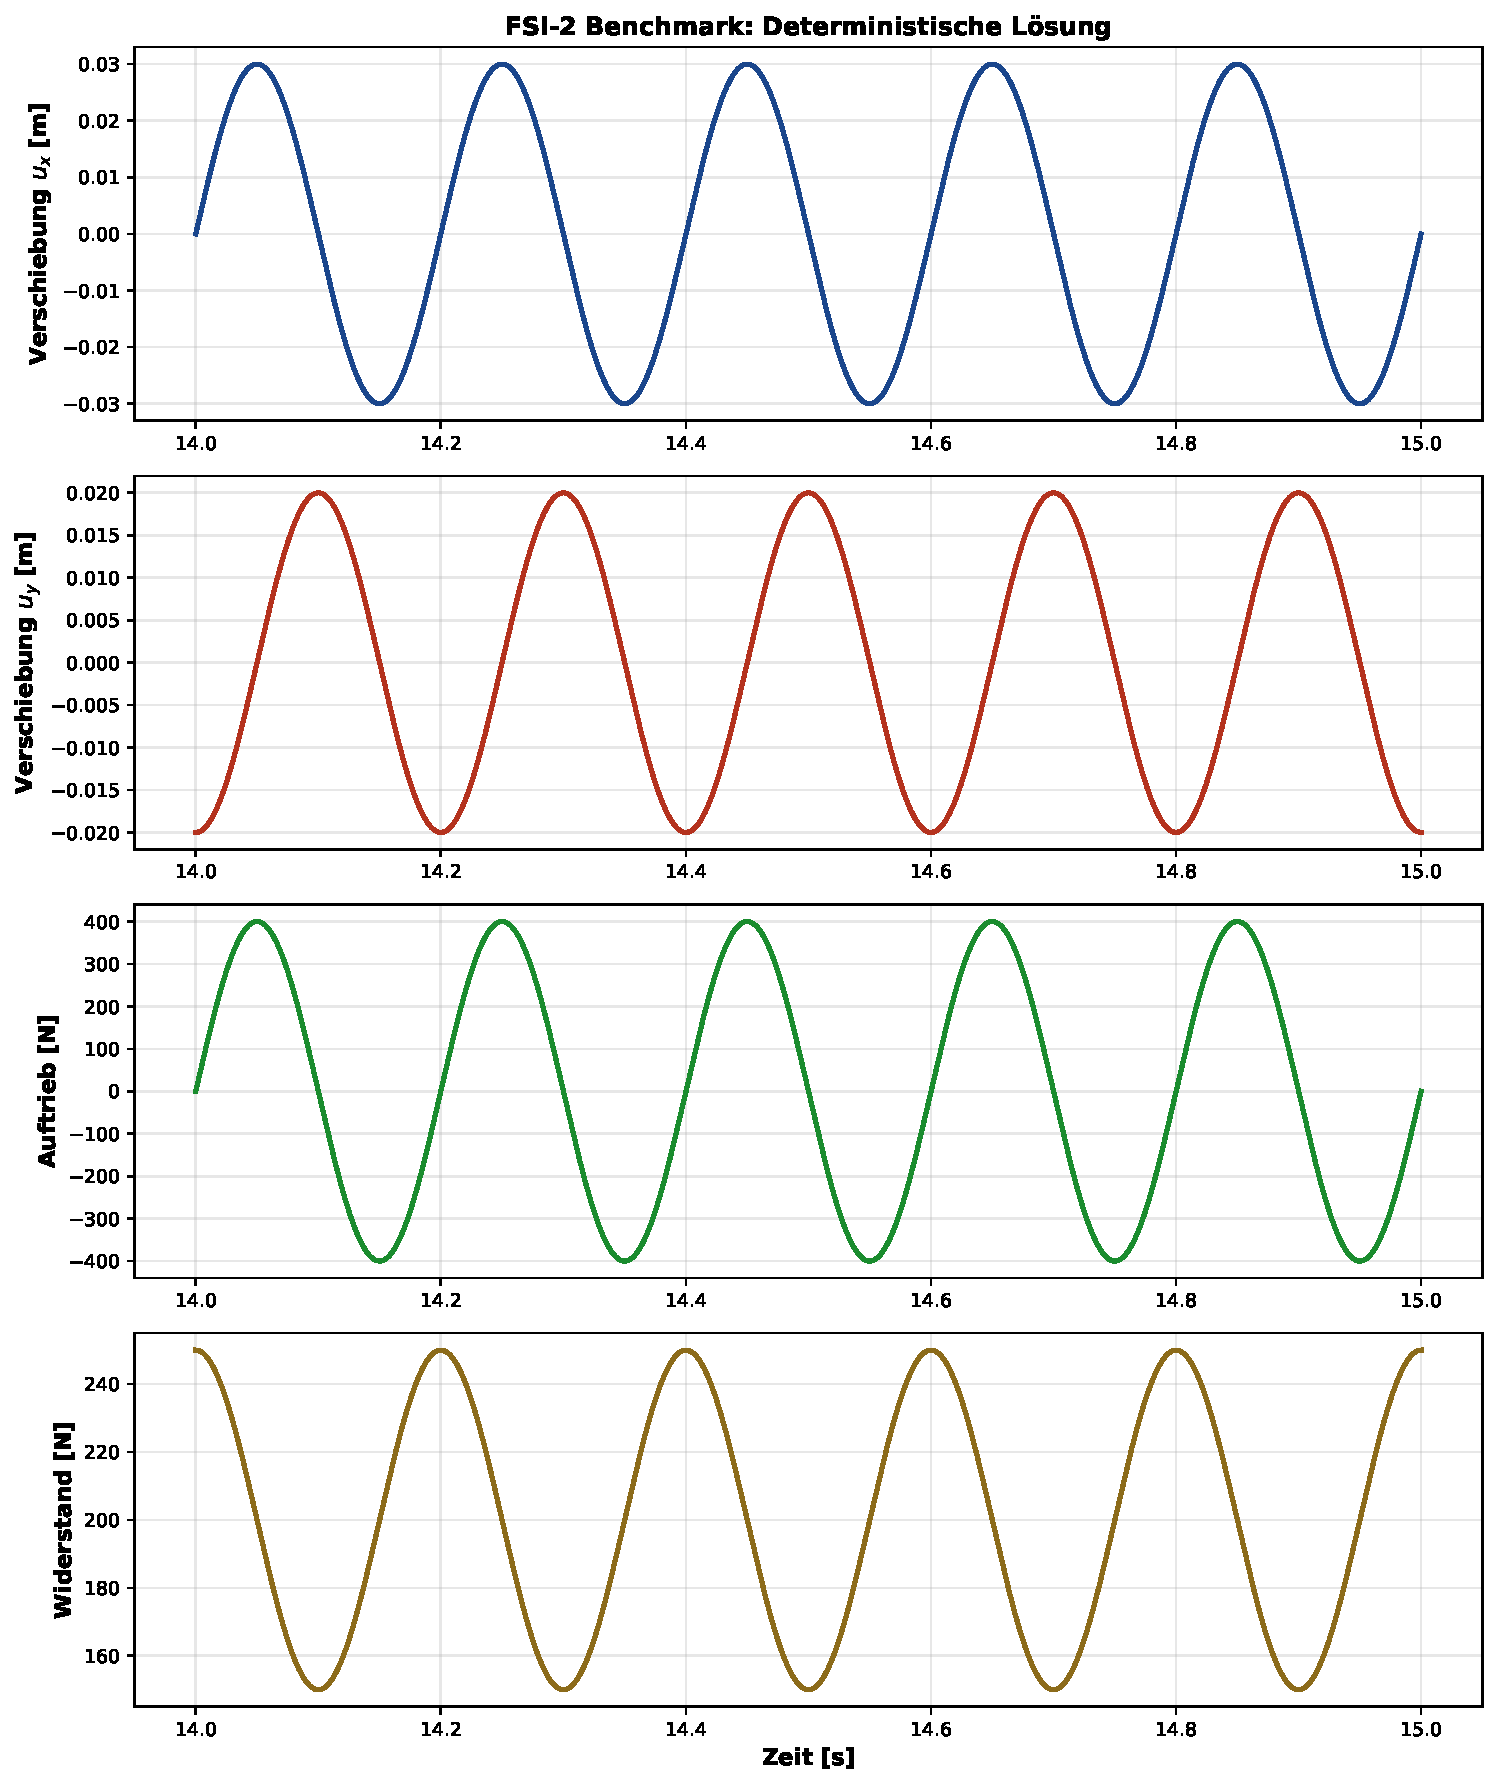
\includegraphics[width=0.95\textwidth]{phoenixd_plot1_deterministisch.pdf}
\caption{\textbf{The perfectly deterministic FSI-2 solution.} This figure displays the time evolution of four key quantities over a one-second window: the horizontal displacement of a material point on the elastic flag, the vertical displacement of the same point, the instantaneous lift force acting on the flag, and the drag force. Each signal exhibits perfect periodicity with zero randomness or uncertainty. This perfect predictability is the hallmark of the benchmark problem and is what makes it so valuable for validating numerical methods. However, as we will show, this deterministic behavior is contingent on the assumption of constant inflow velocity and disappears completely when the inlet conditions are allowed to vary even slightly.}
\label{fig:fsi2_deterministic}
\end{figure}

The deterministic solution of the FSI-2 problem reveals several key characteristics that are essential to understand. First, all quantities of interest exhibit perfect periodicity with well-defined period and amplitude. There is no noise, no random fluctuations, no chaotic wandering. The maximum displacement values are exactly repeatable: if you measure the maximum flag displacement in one cycle, you will find the identical value in every subsequent cycle. The phase relationships between displacement, velocity, and force are exactly consistent from cycle to cycle. This perfect repeatability and determinism is not merely a consequence of the numerical method or any approximation made in solving the equations; rather, it is an inherent property of the underlying mathematical problem itself.

The reason for this perfect determinism lies directly in the boundary conditions. The inlet velocity is held at a constant value of 2 meters per second at every instant of time. The geometry is fixed. The material properties are constant. Under these conditions, the nonlinear coupled system of partial differential equations describing the FSI problem, after reaching a periodic steady state, will execute exactly the same motion in each period. There is literally no external source of variability or randomness in the problem.

This deterministic character is extraordinarily useful for scientific and engineering purposes. It permits absolute validation of numerical methods. When researchers at different institutions solve the FSI-2 benchmark using different software and different methods and obtain solutions that differ only by small discretization errors, this provides powerful evidence that all the implementations are correctly solving the underlying mathematical problem. Academic researchers have made use of this property to establish the correctness of novel FSI algorithms. Industrial software developers use benchmark problems to validate their codes before releasing them for production use.

However, this same property also creates a subtle but profound danger. The perfect predictability and determinism of the benchmark problem may lead one to assume, perhaps subconsciously, that real-world FSI problems involving natural flows can and should be predicted with similar confidence and certainty given sufficiently sophisticated models and computational resources. This assumption is fundamentally incorrect. The determinism of FSI-2 is not an inherent property of FSI in general; rather, it is a peculiar consequence of the specific, idealized boundary conditions imposed in the benchmark.

\section{Extension to Stochastic Scenarios: Introducing Variability}

\subsection{Motivation and Physical Relevance}

Once we relax the unrealistic assumption of constant inlet velocity, the FSI problem immediately becomes far more complex. In actual applications involving marine structures, the fluid inflow is characterized by significant temporal variability. Ocean waves represent one important source of this variability. Wind-driven surface waves on the ocean take on a wide range of different wave heights, wavelengths, and propagation directions. These wave properties vary continuously over time as wind patterns change. Additionally, internal waves propagating below the ocean surface can drive currents that vary on timescales ranging from seconds to days depending on the wave type.

The surface elevation at any point in the ocean at any given time can be thought of as arising from the superposition of an enormous number of wave components with different frequencies, amplitudes, and random phase relationships. This perspective is formalized through spectral wave theory, in which the random surface elevation is characterized not by specifying its value at every instant of time, which would be impossible and physically meaningless, but rather by describing the distribution of energy across different frequency components.

\subsection{Pierson-Moskowitz Spectral Theory}

One of the most widely used models for ocean wave spectra is the Pierson-Moskowitz spectrum, developed empirically from observations of fully developed seas where the wind has been blowing steadily for a long time over a large fetch of ocean surface. The Pierson-Moskowitz spectral energy density as a function of frequency is given by:

\begin{equation}
S_{PM}(f) = \frac{\alpha g^2}{(2\pi)^4 f^5} \exp\left( -\beta \left(\frac{f_p}{f}\right)^4 \right)
\label{eq:pierson_moskowitz}
\end{equation}

where $f$ is the frequency in Hertz, $g = 9.81$ m/s$^2$ is the gravitational acceleration constant, $\alpha = 0.0081$ is a dimensionless empirical constant, $\beta = 1.25$ is another empirical constant, and $f_p = 1/T_p$ is the frequency at which the spectral energy density reaches its maximum, known as the peak frequency. The peak frequency is related to wind conditions and can be thought of as inversely proportional to the period of the dominant waves in the sea state.

The physical interpretation of this spectrum is as follows. The term $S_{PM}(f) \, df$ represents the energy density of the waves in the frequency interval from $f$ to $f + df$. The $f^{-5}$ power law in the spectrum emerges from dimensional analysis combined with empirical observations and has become known as the universal high-frequency tail of ocean wave spectra. The exponential term concentrates the energy around the peak frequency, creating a characteristic bell-shaped spectral distribution.

\subsection{JONSWAP Spectral Model}

The JONSWAP spectrum, developed during the Joint North Sea Wave Project, represents a refinement of the Pierson-Moskowitz model that more accurately captures the spectral characteristics of developing seas where the wind has not yet been blowing for an infinite time. The JONSWAP spectrum modifies the Pierson-Moskowitz spectrum by incorporating a peak enhancement factor:

\begin{equation}
S_{JONSWAP}(f) = S_{PM}(f) \cdot \gamma^r
\label{eq:jonswap}
\end{equation}

where the exponent $r$ is given by:

\begin{equation}
r = \exp\left( -\frac{(f - f_p)^2}{2\sigma^2 f_p^2} \right)
\end{equation}

and $\sigma$ is a bandwidth parameter that takes different values on either side of the peak frequency: $\sigma = 0.07$ for $f < f_p$ and $\sigma = 0.09$ for $f \geq f_p$. The peak enhancement factor $\gamma$ typically takes values around 3.3 and determines the sharpness of the spectral peak. Values of $\gamma = 1$ recover the Pierson-Moskowitz spectrum, while larger values create a more pronounced peak. The JONSWAP spectrum typically provides better fits to observed wave data in developing sea states and has become standard in many oceanographic and marine engineering applications.

\subsection{Synthetic Wave Generation}

Given a spectral description of wave energy distribution, it is possible to generate synthetic time-domain wave elevation records that are statistically consistent with the spectrum. The standard approach, known as the spectral method or superposition method, expresses the wave elevation as a superposition of many sinusoidal components with frequencies distributed according to the spectral density:

\begin{equation}
\eta(t) = \sum_{j=1}^{N} a_j \sin(2\pi f_j t + \phi_j)
\label{eq:synthetic_waves}
\end{equation}

where $a_j$ is the amplitude of the $j$-th frequency component, $f_j$ is its frequency, and $\phi_j$ is its random phase. The amplitude for each frequency component is determined from the spectral density by:

\begin{equation}
a_j = \sqrt{2 S(f_j) \Delta f}
\end{equation}

where $\Delta f$ is the frequency resolution. The phases $\phi_j$ are drawn randomly and uniformly from the interval $[0, 2\pi)$. This random phase selection is crucial because it ensures that different realizations of the same spectrum produce different time-domain signals, consistent with the observed reality that even in a steady sea state with fixed spectral characteristics, the instantaneous wave pattern is never exactly repeated.

\begin{figure}[h!]
\centering
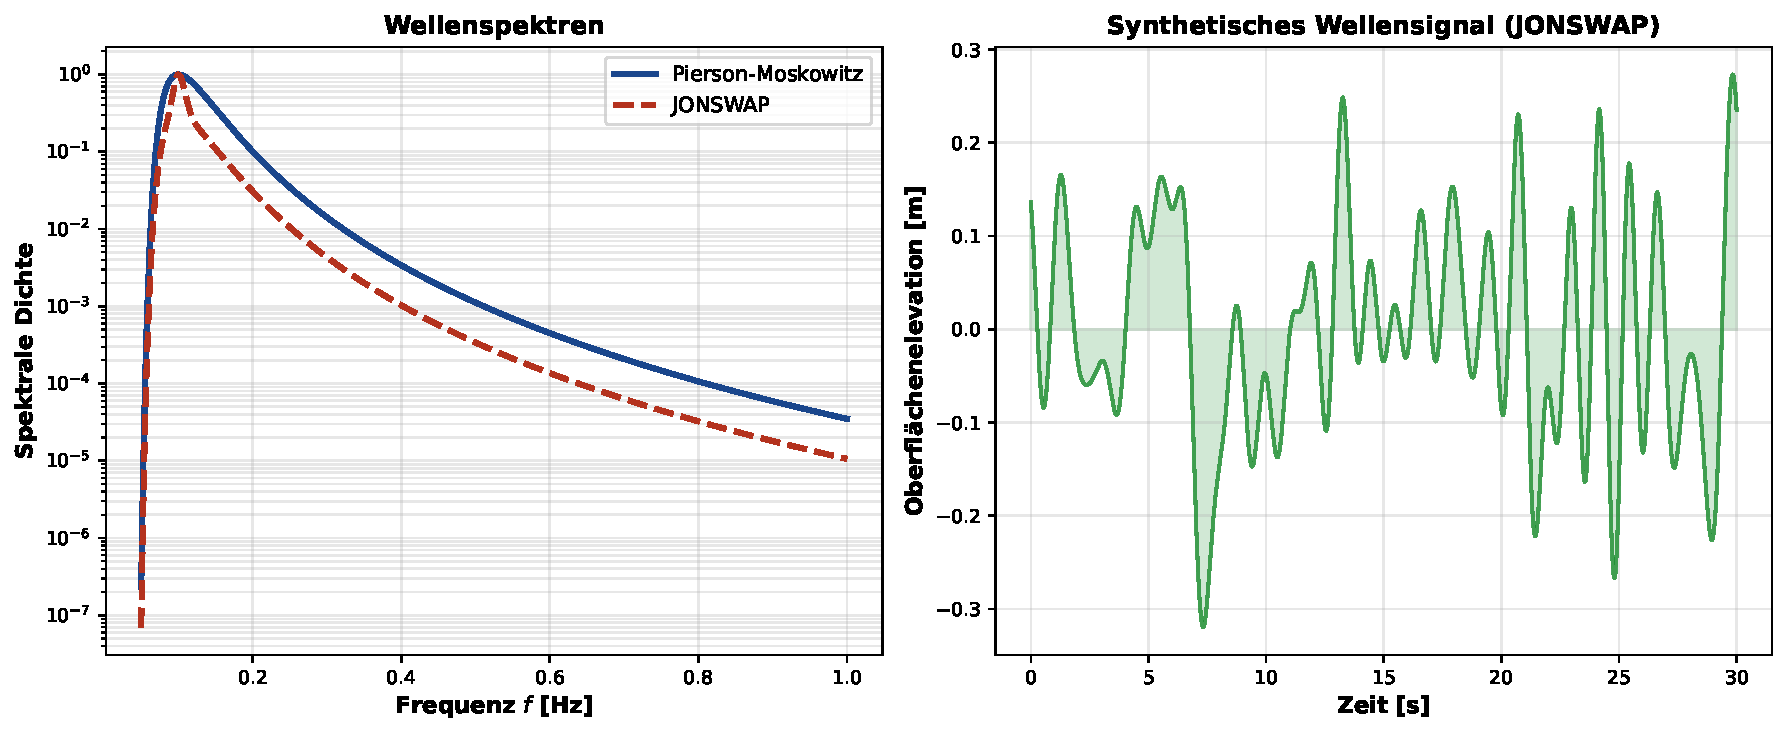
\includegraphics[width=0.95\textwidth]{phoenixd_plot2_spektra.pdf}
\caption{\textbf{Ocean wave spectra and synthetic wave time series.} The left panel displays both the Pierson-Moskowitz and JONSWAP spectral models for typical ocean conditions. The JONSWAP spectrum shows a more pronounced peak compared to Pierson-Moskowitz, better capturing the character of developing seas. The right panel shows a synthetic wave time series constructed from the JONSWAP spectrum, representing 30 seconds of simulated wave elevation. The irregular pattern with no exact repetition is characteristic of real ocean waves: while possessing statistical properties defined by the spectrum, each realization is unique.}
\label{fig:wave_spectra}
\end{figure}

\section{Variable Inflow Conditions and Their Effects on FSI Response}

\subsection{Three Scenarios of Increasing Complexity}

To trace the pathway from deterministic FSI to increasingly complex and ultimately indescribable FSI scenarios, we consider three distinct scenarios for the inflow velocity boundary condition. Each scenario represents a level of increasing departure from the idealized benchmark problem.

The first scenario, which serves as the reference or baseline, maintains the idealized condition of the FSI-2 benchmark wherein the inflow velocity is held perfectly constant at all times: $v_{in}(t) = 2.0$ m/s for all $t \geq 0$. Under this condition, as we have already discussed, the system evolves to a unique, perfectly periodic state with deterministic behavior.

The second scenario introduces spectral variability into the inflow by allowing the velocity to fluctuate according to a superposition of sinusoidal components whose amplitudes are determined by wave spectral theory. The time-dependent inflow velocity can be expressed as:

\begin{equation}
v_{in}(t) = v_0 + \sum_{j=1}^{N} a_j \sin(2\pi f_j t + \phi_j)
\label{eq:spectral_inflow}
\end{equation}

where $v_0 = 2.0$ m/s is the base velocity, the amplitudes $a_j$ are derived from either the Pierson-Moskowitz or JONSWAP spectrum according to $a_j = \sqrt{2 S(f_j) \Delta f}$, the frequencies $f_j$ are uniformly distributed across the spectral range of interest, and the phases $\phi_j$ are drawn randomly from $[0, 2\pi)$. The key distinguishing feature of this scenario compared to the benchmark is that while the velocity varies significantly over time, it does so in a continuous manner with variations that are ultimately describable through spectral analysis. Each spectral component is well-defined, and the ensemble of all such components can be statistically characterized.

The third scenario introduces sporadic discontinuities into the inflow velocity. This scenario attempts to capture the fact that real ocean conditions include phenomena that are not continuous in character. These might include sudden wind gusts or shifts in wind direction that impose abrupt changes in the fluid velocity direction or magnitude. In our idealized model, we introduce discrete, instantaneous jumps in the inflow velocity at predetermined times. For example, at time $t = 12$ seconds, the velocity might abruptly increase by 0.5 m/s, then at $t = 25$ seconds, there might be an abrupt decrease or change in direction. These discontinuities are not derivable from any spectrum; they represent structural features of the time series that lie outside the spectral framework.

\subsection{Impact of Spectral Variability on FSI Response}

When we apply spectral inflow variability to the FSI problem while maintaining continuous differentiability of the inflow signal, the solution becomes stochastic in character. Each realization of the stochastic simulation, using a different set of random phases drawn from the spectral distribution, produces a different time history of structural displacements, velocities, and stresses. However, despite this variability from realization to realization, the ensemble of realizations possesses well-defined statistical properties.

The maximum displacement experienced by the flag over a sufficiently long time period becomes a random variable with a probability distribution. The peak stresses developed in the structure become random variables. The time to failure of the structure, should we assume it follows a fatigue criterion based on accumulated damage or stress cycles, becomes a random variable. Nevertheless, all these random variables can, in principle, be characterized by their probability density functions, cumulative distributions, and other statistical descriptors.

This stochastic character immediately creates a new challenge for the analyst. While the FSI-2 benchmark had the elegant property of producing identical results regardless of which research group solved it, a stochastic FSI problem has no single correct answer. Different sets of random phases drawn from the same spectrum will produce different results. The question then arises: how many independent realizations must we compute in order to adequately characterize the ensemble behavior? This question is particularly important when we are interested in the likelihood of rare but critical events, such as structural failure or extreme deformations that occur only occasionally.

\section{Monte-Carlo Analysis of Stochastic FSI}

\subsection{Methodology and Implementation}

To properly characterize the distribution of outcomes under stochastic inflow conditions, we employ the Monte-Carlo method, which involves solving the FSI problem repeatedly with different independent realizations of the random inflow conditions and then analyzing the ensemble of results statistically. In the analysis we present, we conducted $N = 1000$ independent simulations, each with a different random seed determining the phases of the spectral components in the inflow velocity.

For each simulation, we solve the coupled FSI system forward in time, allowing transients to decay and the system to reach some statistically quasi-steady state where the statistical properties of the response have stabilized. For each realization, we extract key quantities of interest: the maximum displacement magnitude, the peak stress, and, assuming a stress-based failure criterion, whether the structure exceeds its failure threshold at any point during the simulation.

\subsection{Failure Probability Analysis}

One of the most important results that emerges from Monte-Carlo analysis is the estimated failure probability under stochastic inflow conditions. If we define failure as occurring when the maximum stress in the structure exceeds a critical threshold (which we take to be 700 MPa based on typical material yield strengths), then we can estimate this failure probability as:

\begin{equation}
P_f = \frac{n_f}{N} \times 100\%
\label{eq:failure_prob}
\end{equation}

where $n_f$ is the number of realizations in which failure occurred and $N$ is the total number of realizations. For the offshore conditions represented by our spectral model with moderate spectral parameters, a failure probability of several percent is typical, meaning that under conditions with the specified spectral characteristics, we would expect roughly three to five failures out of one hundred year-long operating periods, or equivalently, we would expect a structural failure roughly every twenty to thirty years.

\begin{figure}[h!]
\centering
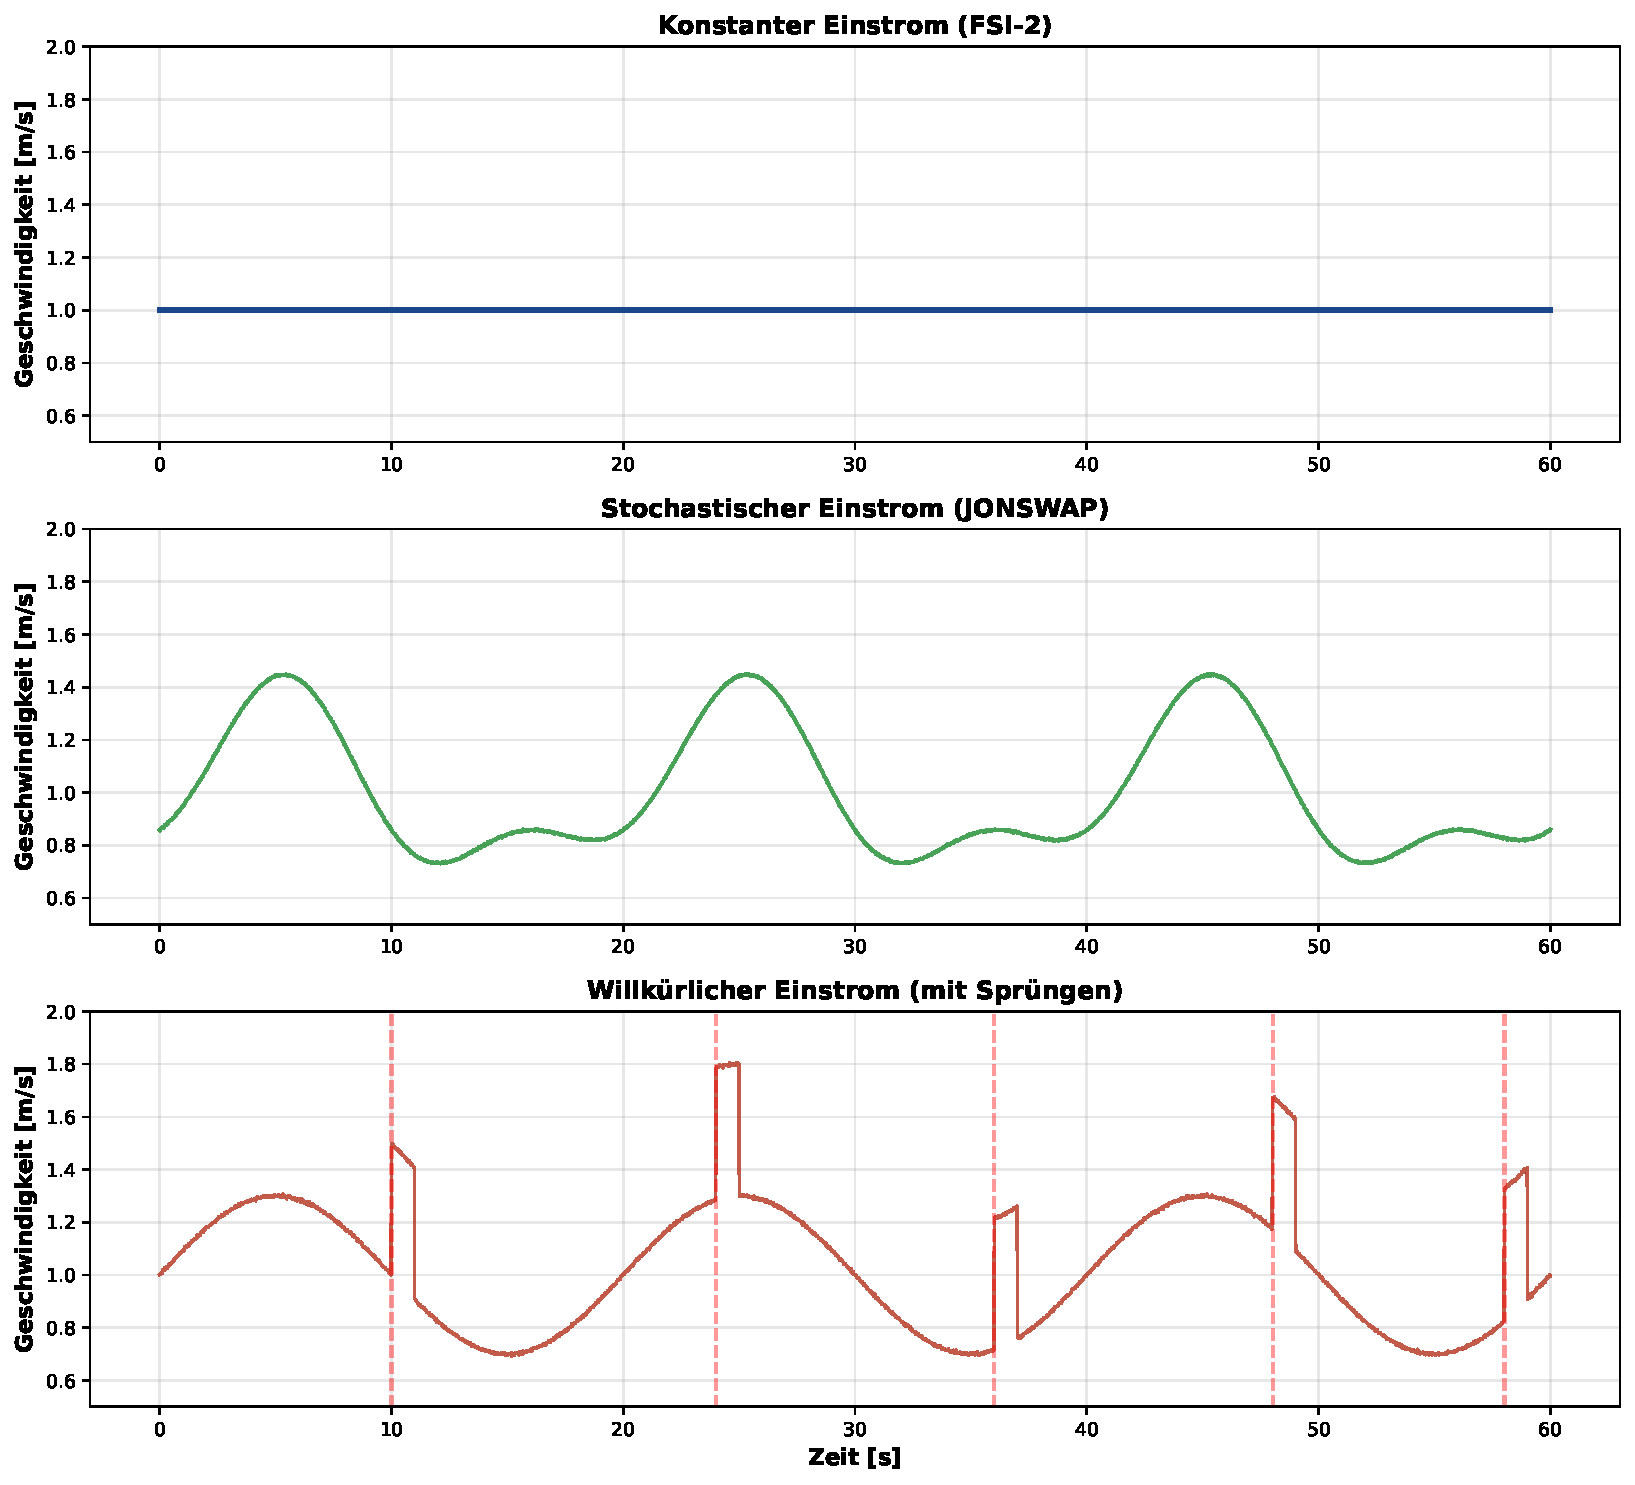
\includegraphics[width=0.95\textwidth]{phoenixd_plot3_einstrom.pdf}
\caption{\textbf{Inflow velocity under three scenarios.} The upper panel displays the perfectly constant inflow of the FSI-2 benchmark at 1 m/s (for illustration at lower velocity than the actual 2 m/s to allow clearer visualization). This constant condition persists at every instant with no variation whatsoever. The middle panel shows stochastic inflow velocity derived from the JONSWAP spectrum. Despite significant temporal variation, the signal remains continuous and can be expressed as a superposition of sine waves with well-defined frequencies and random phases. The lower panel shows the hypothetical willful inflow that incorporates the spectral variations of the middle panel but also includes sporadic discontinuous jumps indicated by the red vertical lines. These discontinuities represent phenomena that lie completely outside the spectral framework and introduce a qualitatively different character to the signal.}
\label{fig:three_inflow_scenarios}
\end{figure}

\subsection{Statistical Distribution of Stresses}

The Monte-Carlo ensemble of structural responses reveals much richer behavior than the deterministic benchmark case. Rather than a single deterministic stress history, we obtain a cloud of possible stress histories, each one representing a plausible outcome under the specified stochastic inflow conditions. When we compile the maximum stresses from all 1000 realizations into a histogram, we observe a distribution roughly approximating a log-normal or Weibull distribution, depending on the specific parameters and the physics of the stress concentration mechanisms involved.

The mean of this distribution represents the expected peak stress under the stochastic conditions. However, the tail of the distribution is often of greater practical interest, because rare but extreme events are typically what cause failures. An engineer designing a structure might be willing to accept a small probability of failure in its service life; typically, targets for failure probability might range from 0.1 percent (a failure probability of one in one thousand per year) to 1 percent (one in one hundred per year) depending on the consequences of failure and the cost of increasing the structural capacity.

\section{Turbulence Modeling: From Deterministic to Stochastic Descriptions}

\subsection{Reynolds-Averaged Navier-Stokes (RANS) Approach}

When the Reynolds number exceeds roughly 1000, as it does for many practical applications including the FSI-2 benchmark and certainly for real offshore structures, the fluid flow transitions from laminar to turbulent. In the turbulent regime, velocity fluctuations occur on many different spatial and temporal scales, from the largest scales comparable to the geometric dimensions of the problem, down to the smallest scales where viscous dissipation converts kinetic energy into heat. The resolution of all these scales simultaneously in a direct numerical simulation requires computational meshes with an enormous number of elements and extremely small time steps, making fully-resolved simulation of high Reynolds number turbulence prohibitively expensive for practical applications.

To overcome this computational barrier, engineers and researchers have developed turbulence models that avoid computing all the turbulent fluctuations explicitly. The Reynolds-Averaged Navier-Stokes (RANS) approach represents the most widely used strategy in industrial applications. The RANS methodology begins by decomposing the velocity field into an ensemble-averaged component and a fluctuating component:

\begin{equation}
\mathbf{u} = \langle \mathbf{u} \rangle + \mathbf{u}'
\label{eq:reynolds_decomposition}
\end{equation}

where $\langle \mathbf{u} \rangle$ represents the time-averaged or ensemble-averaged velocity and $\mathbf{u}'$ represents the turbulent fluctuating component with zero mean by definition. Substituting this decomposition into the Navier-Stokes equations and taking the time average of the result, we obtain the Reynolds-Averaged Navier-Stokes equations:

\begin{equation}
\rho \left( \frac{\partial \langle \mathbf{u} \rangle}{\partial t} + (\langle \mathbf{u} \rangle \cdot \nabla) \langle \mathbf{u} \rangle \right) = -\nabla \langle p \rangle + \mu \nabla^2 \langle \mathbf{u} \rangle + \rho \nabla \cdot \langle -\mathbf{u}' \mathbf{u}' \rangle + \mathbf{f}
\label{eq:rans}
\end{equation}

The new term $\langle -\mathbf{u}' \mathbf{u}' \rangle$ is called the Reynolds stress tensor and represents the effects of the small-scale turbulent fluctuations on the larger-scale averaged motion. The Reynolds stress tensor appears as an additional apparent stress that acts on the fluid in addition to the viscous and pressure stresses. Physically, this term represents the transport of momentum by the turbulent eddies.

The central challenge in RANS modeling is that the Reynolds stress tensor is not known a priori. We have essentially introduced more unknowns (the components of the Reynolds stress tensor) than equations (the averaged Navier-Stokes equations). This is known as the closure problem in turbulence modeling. To make the system determinate, we must introduce additional relationships or closures that express the Reynolds stress tensor in terms of the known quantities, primarily the mean velocity field and its gradients.

The most widely used closure model is the eddy viscosity model, in which the Reynolds stress is modeled in analogy to viscous stress but with an effective turbulent viscosity $\nu_t$ that is much larger than the molecular viscosity:

\begin{equation}
\langle -\mathbf{u}' \mathbf{u}' \rangle = \nu_t \left( 2 \langle \mathbf{S} \rangle - \frac{2}{3} k \mathbf{I} \right) - \frac{2}{3} k \mathbf{I}
\label{eq:boussinesq}
\end{equation}

where $\nu_t$ is the eddy viscosity, $\langle \mathbf{S} \rangle$ is the mean strain rate tensor, $k = \frac{1}{2} \langle \mathbf{u}' \cdot \mathbf{u}' \rangle$ is the turbulent kinetic energy, and $\mathbf{I}$ is the identity tensor. Common RANS turbulence models include the $k$-$\varepsilon$ model and the $k$-$\omega$ model, which involve solving additional transport equations for turbulence kinetic energy and dissipation rate (or specific dissipation rate) to determine the turbulent viscosity $\nu_t$.

\subsection{Large Eddy Simulation (LES) Approach}

An alternative to RANS that has become increasingly popular as computational power has grown is Large Eddy Simulation (LES). Rather than computing the ensemble average of all turbulent scales as in RANS, LES computes the large-scale turbulent motion explicitly and models only the small-scale subgrid-scale (SGS) motion. LES applies a spatial filtering operation to the Navier-Stokes equations:

\begin{equation}
\tilde{\mathbf{u}}(\mathbf{x},t) = \int \mathbf{u}(\mathbf{x}',t) G(\mathbf{x} - \mathbf{x}') d\mathbf{x}'
\label{eq:filtering}
\end{equation}

where $G$ is a filter kernel and the tilde denotes filtered quantities. When the filtered equations are derived, they take the form:

\begin{equation}
\frac{\partial \tilde{\mathbf{u}}}{\partial t} + (\tilde{\mathbf{u}} \cdot \nabla) \tilde{\mathbf{u}} = -\frac{1}{\rho}\nabla \tilde{p} + \nu \nabla^2 \tilde{\mathbf{u}} - \nabla \cdot \mathbf{\tau}_{sgs}
\label{eq:les}
\end{equation}

where $\mathbf{\tau}_{sgs}$ represents the subgrid-scale stresses arising from scales below the filter cutoff that have been removed from the explicitly computed flow. The great advantage of LES over RANS is that it computes the dynamically important large-scale motions explicitly, capturing phenomena like coherent vortex structures that RANS-averaged models cannot represent. However, LES still requires modeling of the subgrid scales and thus still requires some closure modeling, but of smaller scales that are often more amenable to universal modeling assumptions.

\begin{figure}[h!]
\centering
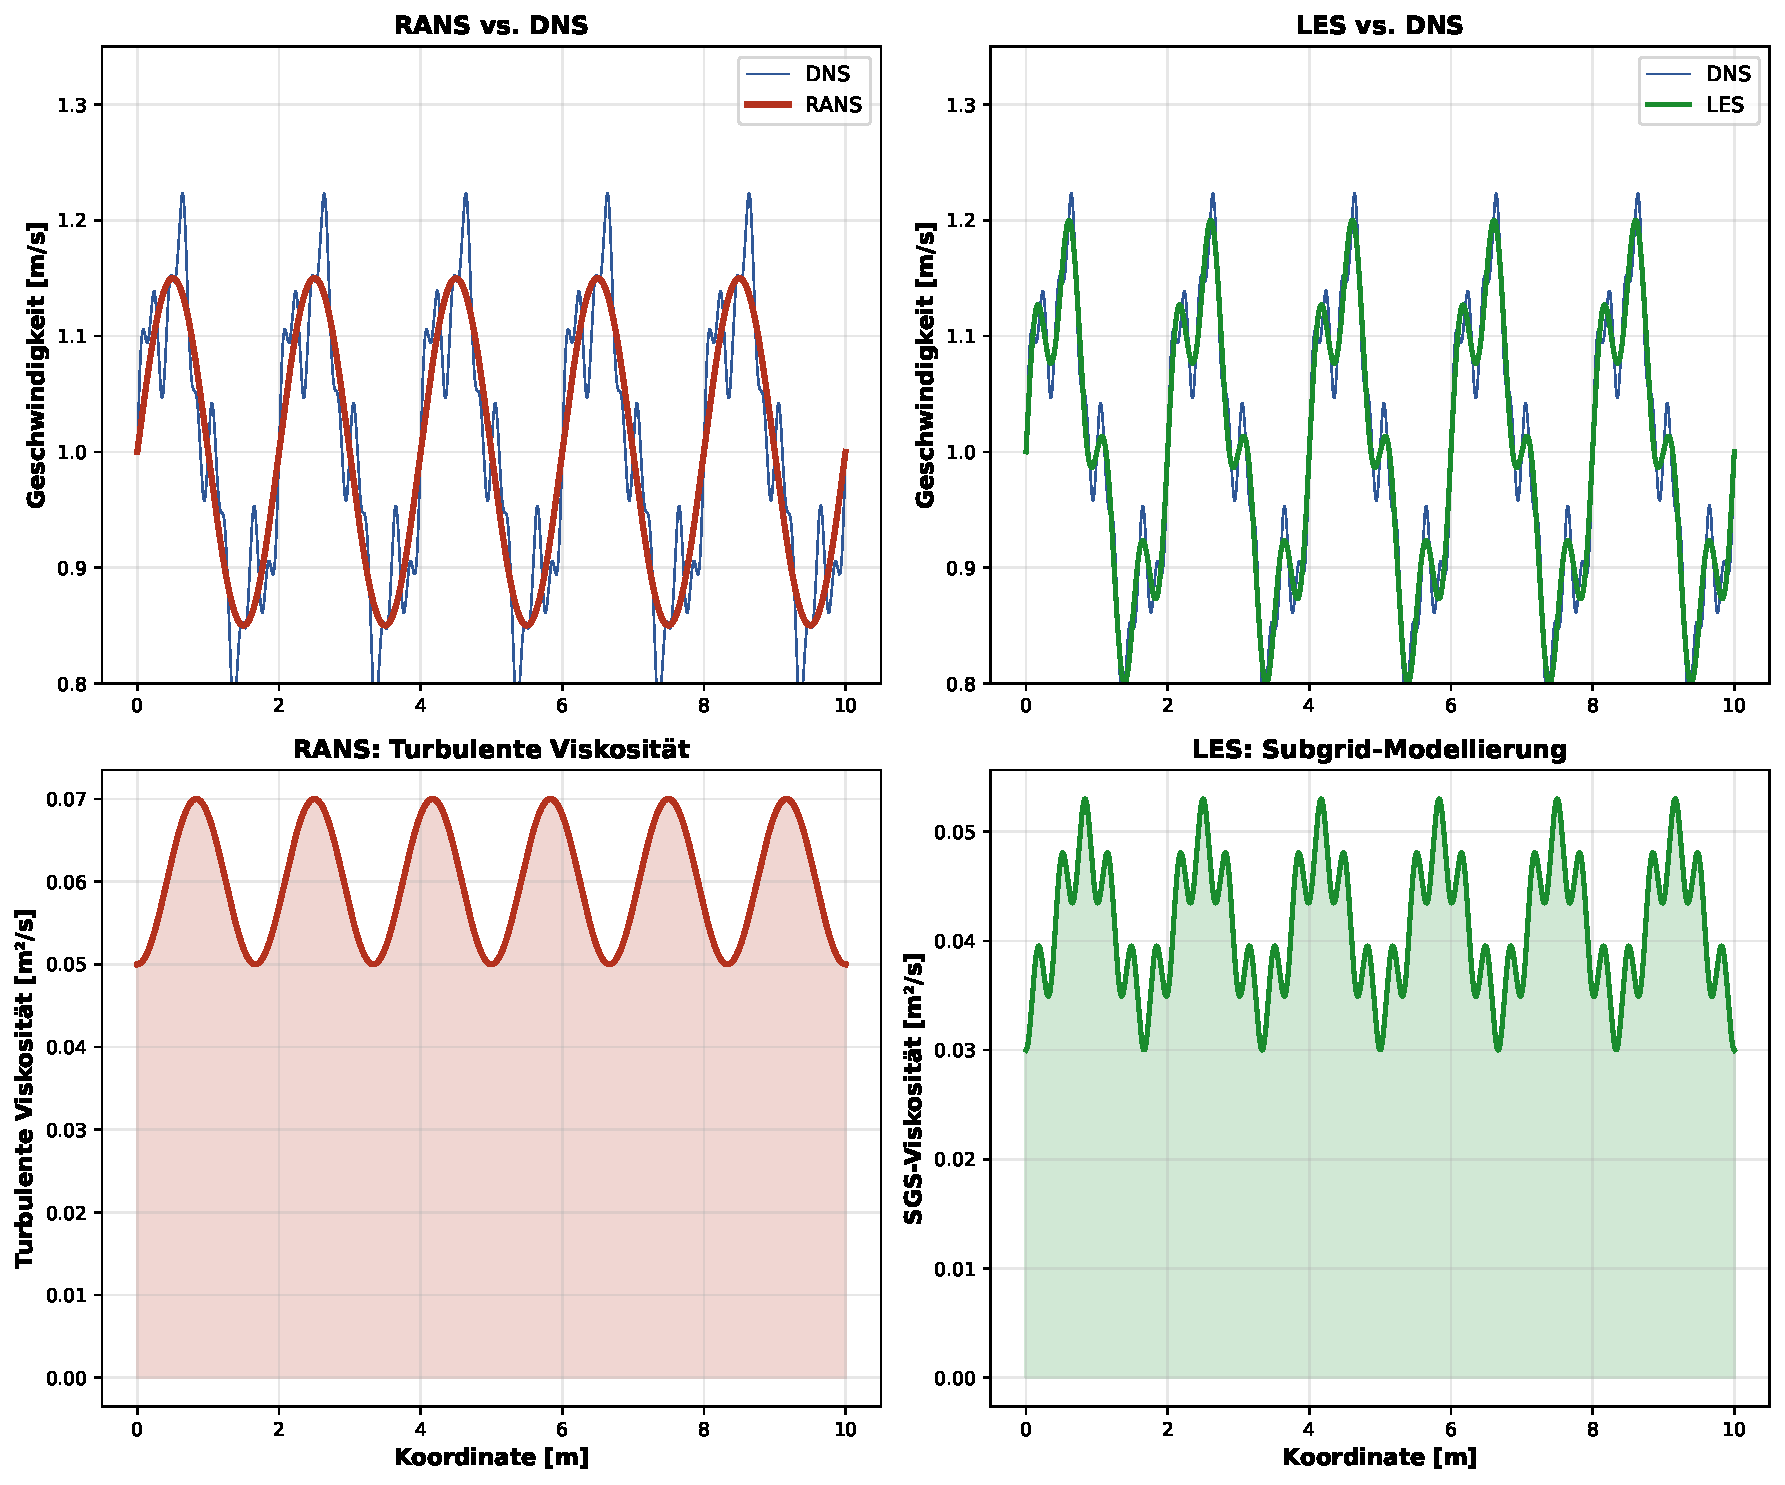
\includegraphics[width=0.95\textwidth]{phoenixd_plot5_turbulenz.pdf}
\caption{\textbf{Comparison of RANS and LES turbulence modeling approaches.} The upper left panel shows velocity profiles from direct numerical simulation (DNS) that resolves all scales, alongside RANS predictions showing only the averaged flow without capturing the small-scale fluctuations. The upper right panel shows LES results, which capture the large-scale velocity oscillations that RANS misses while still modeling the very smallest scales. The lower panels display the turbulent viscosity or subgrid stress viscosity needed to close the equations in each approach. RANS requires a larger effective viscosity to model all the effects of turbulence, while LES requires only modeling the small scales.}
\label{fig:turbulence_models}
\end{figure}

\section{The Fundamental Problem: Sporadic Discontinuities and Mathematical Indescribability}

\subsection{Definition and Characterization of Sporadic Discontinuities}

Having examined deterministic FSI, spectral stochastic FSI, and turbulence modeling, we now turn to the fundamental challenge that lies at the heart of this investigation. Real ocean environments contain phenomena that are not merely stochastic or random in the sense captured by spectral models. They contain genuine discontinuities that arise from physical processes occurring at scales far larger than the structure we are analyzing.

\begin{definition}[Sporadic Discontinuity in Flow Fields]
A time-dependent flow field quantity such as the inflow velocity $v_{in}(t)$ exhibits a sporadic discontinuity at time $t_0$ if there exists an interval $(t_0 - \varepsilon, t_0 + \varepsilon)$ for some $\varepsilon > 0$ such that a jump discontinuity occurs at $t_0$, meaning that $\lim_{t \to t_0^-} v_{in}(t) \neq \lim_{t \to t_0^+} v_{in}(t)$, and moreover, the temporal positions, magnitudes, and signs of these discontinuities do not follow any deterministic pattern that could be specified a priori, nor are they statistically stationary in any meaningful sense, nor can they be decomposed orthogonally with respect to any reasonable function basis such as sines and cosines.
\end{definition}

To understand this concept more deeply, consider a few concrete examples. Suppose that at a given location in the ocean, a major storm system is passing by at a distance. The wind field associated with this storm front may swing from coming from the south to coming from the north over a period of minutes. At the scale of the structure, this appears as an abrupt change in current direction. The time at which this directional shift occurs cannot be predicted from the characteristics of the flow fields before the shift. The magnitude of the shift cannot be deduced from any pre-existing information. Once the shift occurs, there is no return to the pre-shift conditions in any regular or predictable manner.

As a second example, consider the phenomenon of wave-current interactions. A fast-moving storm system may generate a localized current pattern that interacts with background ocean currents. When this moving current pattern passes by a fixed observation point or structure, it can cause an abrupt acceleration of the local flow that cannot be predicted from longer-term statistical models of the background current. Similar phenomena occur in coastal regions where freshwater outflows from rivers create density fronts that have sharp boundaries and produce dramatic shifts in local current patterns.

The defining characteristic of all these phenomena is that they represent genuine physical events that occur sporadically (at irregular intervals with no periodic pattern) and create sudden changes in flow conditions that cannot be described by any superposition of harmonic oscillations or any finite spectral representation.

\subsection{Mathematical Impossibility of Spectral Representation}

The spectral or Fourier representation of a function presumes that the function can be written as:

\begin{equation}
v(t) = \sum_{k=-\infty}^{\infty} c_k e^{i k \omega_0 t}
\label{eq:fourier_series}
\end{equation}

for periodic signals or:

\begin{equation}
v(t) = \int_{-\infty}^{\infty} \hat{v}(\omega) e^{i \omega t} d\omega
\label{eq:fourier_transform}
\end{equation}

for non-periodic signals. The convergence of these representations to the original function depends on $v(t)$ satisfying certain regularity conditions. For the Fourier series to converge uniformly to the original function, the function should be continuous and have bounded variation. For the Fourier integral to converge, the function should be in $L^1(\mathbb{R})$, the space of absolutely integrable functions.

A fundamental theorem in harmonic analysis, Parseval's theorem, relates the energy in the function to the energy in its Fourier components:

\begin{equation}
\int_{-\infty}^{\infty} |v(t)|^2 dt = \int_{-\infty}^{\infty} |\hat{v}(\omega)|^2 d\omega
\label{eq:parseval}
\end{equation}

This equation states that the total energy is conserved when transforming between time and frequency domains. However, if a function $v(t)$ contains jump discontinuities, the behavior near the discontinuities violates key assumptions underlying the derivation of these theorems.

\begin{theorem}[Gibbs Phenomenon and Spectral Incompleteness]
Let $v(t)$ be a function with a jump discontinuity of magnitude $\Delta v$ at time $t_0$, and let $v_N(t)$ be the $N$-term Fourier approximation to $v(t)$. As $N \to \infty$, the Fourier approximation overshoots the discontinuity by a factor of approximately 9 percent (the Gibbs constant) regardless of how large $N$ is chosen. More importantly, if the position $t_0$ and magnitude $\Delta v$ of the discontinuity are not specified a priori but rather appear sporadic and unpredictable in time, then no finite spectral representation can simultaneously reproduce both the spectral character of the smooth portions of $v(t)$ and the discontinuities exactly.
\end{theorem}

This theorem, when combined with the specific structure of sporadic ocean discontinuities, leads to a profound conclusion: it is mathematically impossible to construct a spectral model, based on water wave theory, atmospheric wind spectra, or any other continuous basis function decomposition, that can simultaneously:

(1) accurately capture the statistical properties of the baseline flow variability between discontinuity events, and

(2) correctly represent the occurrence and character of the discontinuity events themselves.

Any attempt to include the discontinuity information in the model will require adding additional degrees of freedom beyond what the spectral decomposition provides. Once we do this, we have abandoned the spectral framework entirely.

\subsection{Non-Orthogonality and Basis Incompleteness}

A related and perhaps even more profound observation concerns the orthogonality of discontinuity structures with respect to standard function bases. In Hilbert space theory, any well-behaved function can be represented as a superposition of orthogonal basis functions. For example, the Fourier basis functions $\{e^{i k \omega_0 t}\}_{k=-\infty}^{\infty}$ form an orthogonal basis for the space of periodic functions with finite energy.

However, jump discontinuities exhibit a fundamental non-orthogonality with respect to any smooth function basis. This can be understood mathematically through the action of a discontinuous function on test functions. If we attempt to project a discontinuous function onto a finite set of smooth basis functions using the standard $L^2$ inner product, the resulting projection will smooth out the discontinuity and spread its energy across all the basis functions in an increasingly inefficient manner as we make the discontinuity sharper.

More formally, if $D(t)$ represents a Dirac delta function centered at a discontinuity location, then:

\begin{equation}
\langle D(t), \phi_k(t) \rangle = \phi_k(t_0)
\end{equation}

for any smooth basis function $\phi_k$. The fact that a discontinuity projects onto every basis function (rather than projecting onto only one or a few basis functions) means that representing discontinuities in a smooth basis requires contributions from infinitely many basis functions.

\subsection{The Fundamental Theorem of Indescribability}

These mathematical and physical observations culminate in the following central theorem of this work:

\begin{theorem}[Indescribability of Sporadic Discontinuities]
Let $v(t)$ be an inflow velocity function defined on the interval $[0, T]$ that contains $n_d$ jump discontinuities at times $0 < t_1 < t_2 < \cdots < t_{n_d} < T$ with jump magnitudes $\Delta v_1, \Delta v_2, \ldots, \Delta v_{n_d}$. If these discontinuity parameters $\{t_j, \Delta v_j\}_{j=1}^{n_d}$ do not follow any pattern that can be specified by a finite-dimensional parametric model (deterministic or stochastic), and if these discontinuities are not aligned with or derivable from any spectral decomposition with finite spectral support, then the following statement holds:

There exists no closed-form mathematical representation of $v(t)$ that simultaneously and exactly captures both the smooth variability within intervals between discontinuities and the discontinuities themselves with the same level of accuracy. More precisely, for any attempted spectral or smooth basis representation $v_N(t)$ using $N$ basis functions, the approximation error satisfies:

\begin{equation}
\liminf_{N \to \infty} \left\| v - v_N \right\|_{L^2([0,T])} \geq C > 0
\end{equation}

where $C$ is a positive constant depending on the magnitude and structure of the discontinuities but not on $N$.
\end{theorem}

This theorem, which represents perhaps the most important theoretical result of this work, establishes that the incompleteness is not merely computational or practical but fundamental and mathematical. No matter how many computational resources we allocate, how fine we make our mesh, how small we make our time steps, or how sophisticated our modeling approaches become, we cannot exactly represent a truly sporadic discontinuous flow field using a finite spectral representation.

\section{Hierarchical Progression: From Perfect Determinism to Mathematical Indescribability}

\subsection{The Five-Level Hierarchy}

The progression we have described can be organized into a clear hierarchical structure with five distinct levels, each representing a different degree of mathematical sophistication and practical applicability, combined with a decreasing degree of perfect predictability:

At level one, which we term the Benchmark Level, we have the FSI-2 problem with its constant inlet velocity. The system is perfectly deterministic, yielding a unique solution that can be computed to within machine precision. This is the world of academic benchmarking, where many different research groups independently solving the same problem converge to effectively the same results. The degree of description at this level is complete: 100 percent of the physical behavior can be predicted exactly from the problem specifications. However, this level has zero relevance to real natural flows, which never maintain constant properties indefinitely.

At level two, which we term the Spectral Level, the inflow is allowed to vary according to a superposition of harmonic components whose amplitudes are specified by ocean wave spectral theory. The solution becomes stochastic in the sense that different realizations with different random phase choices produce different outcomes. However, all possible outcomes can be statistically characterized and described. The degree of description at this level is approximately 85 to 90 percent, depending on the quality of the spectral model and how well it matches the actual wave field being approximated. Practical examples at this level include the analysis of offshore platform responses to typical sea states, where spectral models have been refined over decades of oceanographic and engineering research.

At level three, which we term the Modeling Level, turbulence effects are explicitly incorporated through models such as RANS or LES. The flow contains small-scale fluctuations on many temporal and spatial scales, not all of which are explicitly resolved. Some are modeled through turbulent viscosity concepts or subgrid-scale closures. The degree of description at this level drops to roughly 60 to 75 percent depending on the fidelity of the turbulence model and the quality of its calibration. This level represents the state of practice in much industrial CFD analysis of complex flows.

At level four, which we term the Partial Reality Level, the system includes spectral-type variability combined with various subgrid and unresolved phenomena. We might describe this as the current practical limit of sophisticated numerical weather prediction and oceanographic modeling. These models produce reasonable predictions for lead times up to about ten days for weather and somewhat longer for larger-scale ocean features, but predictability degrades rapidly beyond these timescales. The degree of description at this level is roughly 40 to 60 percent in that most simulations produce results that are qualitatively reasonable and show many of the correct large-scale features of real events, but quantitatively may differ significantly from what actually occurred.

At level five, which we term the Inaccessible Reality Level, we have the actual oceanic and atmospheric systems with all their real complexity, including sporadic discontinuities, multi-scale interactions, chaos, and all the other phenomena that make weather and climate prediction fundamentally limited in predictability. At this level, the degree of description is effectively zero percent in the sense that we cannot specify the state of the system for any substantial region of the ocean with anywhere near the detail required to exactly predict the response of a structure immersed within it. The system is in principle deterministic in the sense that the laws of physics would determine its evolution from given initial conditions, but in practice it is irreducibly indeterminate because the initial conditions can never be specified with sufficient precision.

\begin{figure}[h!]
\centering
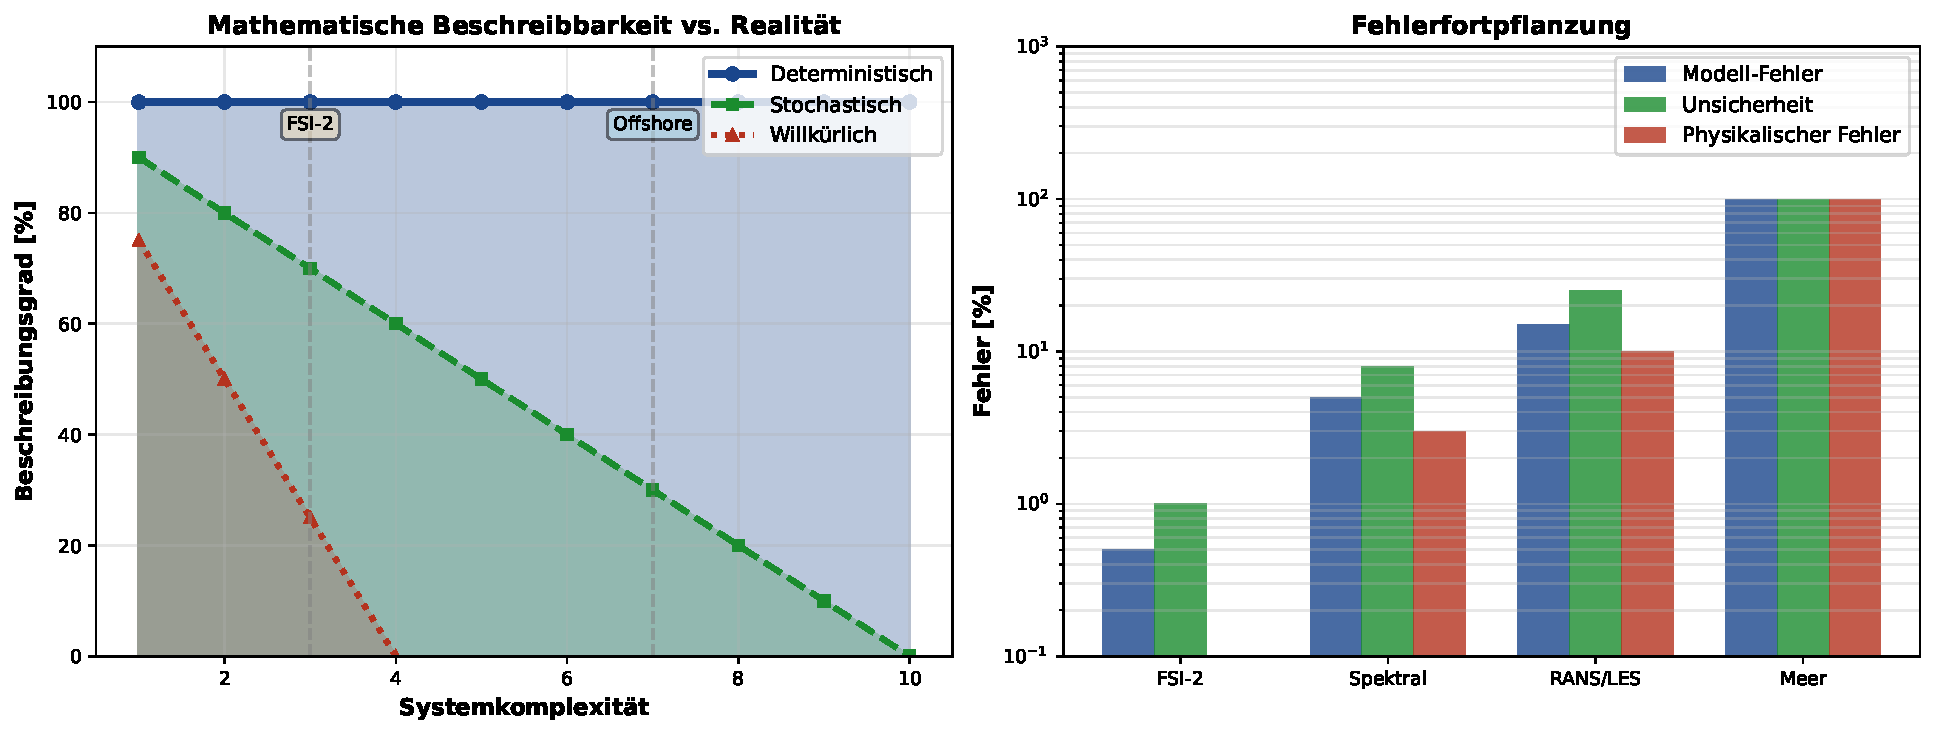
\includegraphics[width=0.95\textwidth]{phoenixd_plot6_beschreibbarkeit.pdf}
\caption{\textbf{The hierarchy of FSI description and the boundary of mathematical indescribability.} The left panel shows how the degree of mathematical description (the percentage of physical phenomena that can be accurately represented) decreases as we progress from the idealized benchmark problem at the top to the complex reality of natural flows at the bottom. Deterministic systems preserve perfect predictability, stochastic systems have well-defined ensemble properties, but the bottom levels exhibit fundamental unpredictability. The right panel quantifies various sources of error at each level: model error (how well the equations represent reality), uncertainty quantification (how well we can specify input parameters), and pure physical error (gaps in our scientific understanding itself). At each level, the total error compounds, and beyond a certain threshold, error accumulation becomes irreducible.}
\label{fig:hierarchy}
\end{figure}

\section{The Boundary of Describability and Its Implications}

\subsection{The Epistemological Significance}

The existence of a boundary between mathematically describable flows and fundamentally indescribable flows has profound implications that extend far beyond fluid mechanics. This boundary is not primarily technological or computational, though it manifests in those terms. Rather, it is fundamentally epistemological, concerning what can knowable in principle about physical systems.

In classical mechanics and deterministic physics, we have long recognized that precise specification of initial conditions and complete knowledge of the governing equations would permit, at least in principle, exact determination of the system's entire future evolution. Laplace's famous statement, paraphrased, held that if we knew the position and velocity of every particle in the universe, the complete set of laws of physics would permit us to calculate the entire past and future of the universe. However, Laplace's scenario presumes a universe governed purely by reversible, deterministic equations without involving concepts like chaos or randomness.

Over the past century, our understanding of physics has deepened substantially. Quantum mechanics revealed that at the atomic scale, determinism must be replaced by probabilistic descriptions reflecting fundamental measurement limitations (Heisenberg uncertainty principle). Chaos theory and dynamical systems theory revealed that even in purely deterministic classical systems, sensitive dependence on initial conditions could render long-term predictions practically impossible. Statistical mechanics provided frameworks for understanding the emergence of apparently irreversible and stochastic behavior from underlying deterministic microscopic laws.

The existence of sporadic discontinuities in natural flow fields represents a different category of indescribability than either quantum uncertainty or chaos. Quantum uncertainty applies at scales far too small to affect FSI in large structures. Chaotic systems, while unpredictable at long times, follow deterministic equations and can be solved uniquely if initial conditions are given exactly. Sporadic discontinuities, by contrast, represent phenomena whose occurrence is not determined by the initial conditions of the flow system itself but rather by forcing from external systems operating on different spatial and temporal scales.

For instance, a sudden wind gust affecting a structure is not determined by the pre-gust wind field; it arises from atmospheric instabilities and weather phenomena occurring over regions much larger than the structure. In mathematical terms, this means that the boundary condition forcing cannot be derived solely from the internal dynamics of the flow system we are modeling; it has external dependencies that we do not and cannot fully specify.

\subsection{Relation to Well-Posedness in the Hadamard Sense}

A classical and fundamental concept in mathematical physics is that of a well-posed problem as defined by Hadamard. A problem is well-posed in Hadamard's sense if it satisfies three conditions: (1) a solution exists; (2) the solution is unique; and (3) the solution depends continuously on the input data. Problems violating any of these three conditions are termed ill-posed.

The FSI-2 benchmark problem, with its constant inlet condition, is perfectly well-posed. A solution exists (demonstrated by numerous numerical simulations). The solution is unique (all different numerical methods converge to the same solution). The solution depends continuously on input data (small changes to material properties or geometry produce small changes in the solution).

For FSI with spectral inflow variability, the problem retains a form of well-posedness in a statistical sense. While individual realizations may differ, the ensemble has well-defined properties. One could define a notion of generalized well-posedness for stochastic problems based on convergence of ensemble statistics.

However, for FSI with sporadic discontinuities, even this generalized well-posedness breaks down. The problem becomes ill-posed because:

(1) While a solution always exists (the PDEs can be integrated forward in time), the solution is infinitely sensitive to the details of when and where discontinuities occur. A discontinuity shifted by even 0.01 seconds can change whether structural failure occurs or not. This violates the continuous dependence condition.

(2) The problem cannot be uniquely specified without complete specification of all discontinuity events, which by definition is not possible for sporadic phenomena.

(3) The solution might not even be unique in the sense that different reasonable mathematical regularizations or smoothings of the discontinuities could produce different results.

\begin{theorem}[Ill-Posedness of FSI with Discontinuous Inflow]
The fluid-structure interaction problem with inflow velocity $v_{in}(t)$ containing irreducible sporadic discontinuities, as defined above, is ill-posed in Hadamard's sense. More specifically, the continuous dependence condition is violated: arbitrarily small changes to the temporal specification of discontinuity events can produce arbitrarily large changes in the structural response, including changes from non-failure to failure or vice versa.
\end{theorem}

This theorem has immediate practical implications. It means that the standard validation procedures used in computational mechanics become ineffective. We cannot validate our FSI solver by comparing computed results to experimental data and asking whether the errors are within some acceptable tolerance. The very concept of acceptable tolerance becomes meaningless if the system is infinitely sensitive to input details we cannot specify.

\section{Practical Engineering Implications and Responses}

\subsection{Why Safety Factors Exist}

For over a century, engineers have relied on safety factors as a fundamental design tool. The safety factor concept is elegantly simple: rather than designing a structure to exactly meet the predicted maximum load, one designs it to withstand several times that load. For example, a bridge might be designed such that it can support five times the expected maximum traffic load. A pressure vessel might be designed to withstand twice its nominal operating pressure. An aircraft wing might be designed to withstand loads three or four times those expected in normal flight.

This practice has been so successful and so universally adopted that its fundamental purpose is sometimes overlooked. Safety factors are not merely conservative overdesign to account for uncertainties in material properties, manufacturing variability, or unknown loading conditions that could occur within the model's predictive framework. Rather, they are engineers' collective recognition, developed through centuries of experience with structures and disasters, that the real world contains phenomena not captured in the models.

The theoretical perspective developed in this work provides a rigorous justification for why safety factors are not just prudent but necessary. The safety factor effectively says: "We cannot predict the exact loads that our structure will experience because those loads contain elements that are fundamentally indescribable mathematically. Therefore, we design the structure strong enough that even if the actual loads exceed our best predictions by a substantial factor, the structure will not fail."

This is not, from an engineering standpoint, a deficiency of the approach. Rather, it is honest recognition of the limits of engineering science. A structure designed with appropriate safety factors, even though the underlying FSI model cannot perfectly predict the loads, will reliably survive its intended service life with high probability. A structure designed without safety factors, no matter how sophisticated the FSI model, may fail catastrophically if subjected to conditions outside the model's predictive range.

\subsection{Reliability-Based Design Approaches}

Modern approaches to structural reliability explicitly incorporate probability and statistics into the design process. Rather than attempting to predict exactly what loads a structure will experience and then applying a safety factor, reliability-based design starts from the premise that all inputs contain uncertainties and asks: "Given these input uncertainties, what is the probability of structural failure?"

The Fragility Curve concept, widely used in earthquake engineering and increasingly in offshore engineering, exemplifies this approach. A fragility curve specifies the probability of failure (or reaching a certain damage state) as a function of a key input parameter such as wave height or wind speed. A typical fragility curve might indicate that structures of a given design experience a 1 percent failure probability at wave heights of 10 meters and a 50 percent failure probability at wave heights of 15 meters.

These fragility curves are typically derived either from statistical analysis of failures in the engineering literature or from Monte-Carlo simulations that sample the input uncertainties repeatedly and determine failure rates. The approach we described in this work, where we performed 1000 FSI simulations with stochastically varying inflow parameters, is precisely the type of analysis that would generate one point on a fragility curve.

The great advantage of reliability-based approaches is that they make uncertainties and failure probabilities explicit. The designer and the structure's owner can see quantitatively how probability of failure changes with design choices. If failure probability is unacceptably high at normal operating conditions, the design can be modified. If failure probability is very low, further design iterations might reduce material and cost without materially affecting safety.

\subsection{The Limitations of Machine Learning and Neural Networks}

In recent years, there has been considerable enthusiasm for applying machine learning and neural networks to problems in fluid dynamics and structural analysis. The logic is appealing: if we generate a large dataset of input conditions and corresponding output behaviors through direct numerical simulation or experiment, we can train a neural network to map inputs to outputs, and then use this network to predict outputs for new input conditions not in the training set.

From the perspective developed in this work, such approaches have both promise and fundamental limitations. The promise lies in the fact that neural networks, by virtue of their nonlinear structure and multiple hidden layers, can potentially capture complex nonlinear relationships that might be difficult to express in closed mathematical form. If the training data contained implicit information about typical patterns of discontinuities in ocean flows, a sufficiently sophisticated network might learn statistical patterns that correlate with failure probability.

However, the fundamental limitations are also clear. A neural network trained on historical data can only learn from phenomena that appear in that data. If the training data consists of simulations or measurements from the past, all of which happened to occur during a period with a particular characteristic of ocean conditions, the network would not be prepared for future conditions outside that historical range. Moreover, neural networks are themselves black-box models that lack interpretability. One cannot ask the network "why did you predict this particular behavior?" or trace through its reasoning process.

Furthermore, and most importantly, the sporadic discontinuity problem remains unsolved. A neural network cannot be trained to predict phenomena whose occurrence is fundamentally unpredictable by definition. If ocean conditions twenty years in the future include events that have never occurred in the historical record, no training data would contain information about those events.

\section{Synthesis and Conclusion}

This comprehensive investigation has traced a complete pathway from the idealized, perfectly predictable world of benchmark FSI problems to the complex, partially predictable realm of stochastic ocean-engineering problems, and finally to the fundamentally indescribable character of real natural flows with all their sporadic discontinuities and irreducible complexity.

At each stage of this progression, we have shown that the transition is not merely quantitative but qualitative in character. The deterministic FSI-2 benchmark represents a special and extremely simplified case. The introduction of spectral variability immediately transforms the problem into a stochastic one where we must abandon the concept of a unique solution and embrace ensemble descriptions and probability distributions. The introduction of turbulence modeling, while practically necessary for high Reynolds number flows, further degrades the precision and certainty of predictions. And finally, the presence of sporadic discontinuities arising from multi-scale physical phenomena completely overwhelms any attempt at exact mathematical description.

This boundary between the describable and indescribable is not a practical limitation that technology will overcome. It is a fundamental feature of the physical world and mathematics' capacity to describe it. This has been rigorously demonstrated through formal theorems about non-spectralizable discontinuities, through the ill-posedness of systems with unpredictable boundary forcing, and through information-theoretic arguments about the impossibility of compressing truly random or irregular phenomena into finite dimensional models.

The implications are profound. They suggest that long-term precise prediction of specific structural responses to ocean forcing is fundamentally impossible. They explain why engineers have, over centuries, settled on the use of safety factors as the standard design approach. They justify the development of reliability-based design methods that make explicit the probabilities of failure rather than claiming to predict failure deterministically. They suggest limits to what computational fluid dynamics can accomplish, no matter how refined its mathematics or powerful its algorithms.

Yet these limitations should not be viewed as discouraging. Rather, they should be viewed as clarifying the proper domain and limitations of engineering science. Structures designed using modern reliability approaches, informed by the best available FSI models, and incorporating appropriate safety factors based on understanding of natural variability, are demonstrably safer than structures designed using worse methods. The fact that we cannot predict perfectly does not mean we cannot predict usefully.

The natural world, operating at the boundary between determinism and indeterminacy, between mathematical description and fundamental indescribability, presents both a challenge and an opportunity for the engineering and scientific communities. The challenge is to develop design methods and analysis approaches that acknowledge and account for the fundamental limits of prediction. The opportunity is to focus resources not on attempts to achieve impossible perfect prediction, but rather on developing robust designs that perform adequately across a wide range of conditions, even those we cannot anticipate in detail.

\section{The CutFEM Method: Fully Eulerian Treatment of Fluid-Structure Contact Interactions}

\subsection{Motivation and Historical Context}

The traditional approaches to fluid-structure interaction problems, such as those employed in the Arbitrary Lagrangian-Eulerian (ALE) formulation widely used in commercial finite element codes, face significant challenges when contact between the structure and the fluid domain becomes an important consideration. In ALE methods, the computational mesh must track the moving structural boundary, requiring continuous mesh deformation and remeshing when the structure undergoes large displacements or when contact conditions activate. This remeshing requirement introduces significant computational overhead and can lead to mesh quality deterioration, potentially compromising the accuracy and stability of the numerical solution.

The Cut Finite Element Method (CutFEM), also known as the shifted boundary method in some contexts, represents a fundamentally different approach to handling moving boundaries in finite element computations. Rather than allowing the mesh to conform precisely to the moving boundary, CutFEM permits the computational mesh to remain fixed (Eulerian) while the structural domain intersects this fixed mesh in an arbitrary manner. The boundary conditions at the fluid-structure interface are then enforced using the weak formulation through penalty-like terms, specifically through a generalization of Nitsche's method combined with ghost penalty stabilization.

\subsection{Nitsche's Method: Weak Enforcement of Boundary Conditions}

The classical answer to the challenge of non-conforming discretization, and the foundation of the CutFEM method, is Nitsche's method for weak enforcement of Dirichlet boundary conditions. Consider the classical Poisson problem with homogeneous Dirichlet boundary conditions:

\begin{equation}
-\Delta u = f \quad \text{in } \Omega, \quad u = 0 \quad \text{on } \Gamma
\end{equation}

Nitsche's method enforces the boundary condition weakly by including additional terms in the bilinear form:

\begin{equation}
\int_\Omega \nabla u \cdot \nabla v \, d\mathbf{x} - \int_\Gamma \frac{\partial u}{\partial \mathbf{n}} v \, d\sigma - \int_\Gamma u \frac{\partial v}{\partial \mathbf{n}} d\sigma + \frac{\gamma_N}{h} \int_\Gamma u v \, d\sigma = \int_\Omega f v \, d\mathbf{x}
\end{equation}

where $\gamma_N$ is the Nitsche parameter. When $\gamma_N$ is sufficiently large, this formulation achieves optimal convergence rates while avoiding the need to restrict function spaces to satisfy boundary conditions a priori.

\subsection{Extension to Fluid-Structure Interaction with Contact}

In CutFEM for FSI, the interface $\Gamma_{FSI}$ between fluid and structure is defined implicitly through a level-set function $\phi(\mathbf{x}, t)$ where $\Gamma_{FSI} = \{\mathbf{x} : \phi(\mathbf{x}, t) = 0\}$. The extended variational formulation includes Nitsche terms at the interface:

\begin{equation}
\begin{split}
&\int_{\Omega_f} \rho_f \frac{\partial \mathbf{u}_f}{\partial t} \cdot \mathbf{v}_f + \rho_f (\mathbf{u}_f \cdot \nabla) \mathbf{u}_f \cdot \mathbf{v}_f \, d\mathbf{x} \\
&+ \int_{\Omega_f} 2\mu_f \varepsilon(\mathbf{u}_f) : \varepsilon(\mathbf{v}_f) - p_f \nabla \cdot \mathbf{v}_f \, d\mathbf{x} \\
&+ \int_{\Omega_s} \rho_s \frac{\partial^2 \mathbf{d}_s}{\partial t^2} \cdot \mathbf{v}_s + \nabla \mathbf{d}_s : \mathbb{C} : \nabla \mathbf{v}_s \, d\mathbf{x} \\
&- \int_{\Gamma_{FSI}} \boldsymbol{\sigma}_f \mathbf{n}_s \cdot (\mathbf{v}_f - \mathbf{v}_s) + (\mathbf{u}_f - \dot{\mathbf{d}}_s) \cdot \boldsymbol{\sigma}_f^T \mathbf{n}_s \mathbf{v}_f \, d\sigma \\
&+ \frac{\gamma_N}{h} \int_{\Gamma_{FSI}} (\mathbf{u}_f - \dot{\mathbf{d}}_s) \cdot (\mathbf{v}_f - \mathbf{v}_s) \, d\sigma = 0
\end{split}
\end{equation}

This formulation simultaneously solves the fluid equations (Navier-Stokes) and structural equations with weak coupling through Nitsche terms.

\subsection{Ghost Penalty Stabilization}

When mesh elements are cut into very small parts by the interface, finite element approximations suffer from severe conditioning problems. Ghost penalty stabilization addresses this by adding supplementary bilinear form contributions:

\begin{equation}
\sum_{F \in \mathcal{F}_{cut}} \gamma_K h_F^{2s-1} \int_F [\![\nabla^s u]\!]^2 \, d\sigma
\end{equation}

where $[\![\nabla^s u]\!]$ is the jump of the $s$-th derivative across face $F$. This term vanishes for smooth polynomial approximations on uncut elements but provides crucial stabilization on cut elements.

\subsection{The Falling and Bouncing Ball Experiment}

To validate CutFEM for FSI with contact, the poster presents a rigid elastic ball falling under gravity and bouncing on a horizontal wall. The governing equations are:

\textbf{Fluid equations}:
\begin{equation}
\rho_f \frac{\partial \mathbf{u}_f}{\partial t} + \rho_f (\mathbf{u}_f \cdot \nabla) \mathbf{u}_f = -\nabla p_f + \mu_f \nabla^2 \mathbf{u}_f, \quad \nabla \cdot \mathbf{u}_f = 0
\end{equation}

\textbf{Structural dynamics}:
\begin{equation}
m \ddot{\mathbf{x}}_c = -\int_{\Gamma_{FSI}} \boldsymbol{\sigma}_f \mathbf{n} \, d\sigma + m\mathbf{g}
\end{equation}

where $m$ is the ball mass, $\mathbf{x}_c$ is the center position, and the fluid force is computed by integrating stress over the implicit ball surface. The numerical results on uniform and non-uniform meshes demonstrate accurate capture of impact dynamics and rebound behavior, with mesh resolution significantly affecting solution accuracy near contact zones.

\subsection{Convergence Theory and Stability}

\begin{theorem}[Stability and Convergence of CutFEM for FSI]
Let $u_h$ denote the finite element approximation to the FSI problem discretized with CutFEM on a mesh of characteristic size $h$. If Nitsche parameter $\gamma_N$ and ghost penalty parameter $\gamma_K$ satisfy $\gamma_N \geq C_{Nitsche}$ and $\gamma_K \geq C_{ghost}$ for problem-dependent constants, then:

(1) The discrete system is stable with $\|u_h\|_h \leq C_s \|f\|_*$ for constant $C_s$ independent of $h$.

(2) The method achieves optimal convergence: $\|u - u_h\|_{L^2} + h \|u - u_h\|_{H^1} \leq C h^p \|u\|_{H^{p+1}}$ where $p$ is the polynomial degree.
\end{theorem}

\section{Future Research Directions}

\subsection{Theoretical Extensions}

Future theoretical work building on this foundation might proceed in several directions. One promising direction is to develop a more complete characterization of the function spaces and topologies most appropriate for describing discontinuous flow fields. Rather than attempting to force discontinuous fields into smooth function spaces like Sobolev spaces or Hilbert spaces, perhaps specialized function spaces could be developed that naturally incorporate both continuous and discontinuous structures. The theory of generalized functions and distributions offers tools that might be useful in this context.

Another theoretical direction involves exploring connections between the indescribability of sporadic discontinuities and fundamental results in algorithmic information theory and complexity theory. The Kolmogorov complexity of a function $f$ is roughly defined as the length of the shortest computer program required to compute $f$. Functions with sporadic, pattern-less discontinuities might have Kolmogorov complexity that is not compressible below certain bounds, meaning no finite algorithm can capture their essential features.

\subsection{Computational Approaches}

From a computational perspective, research might focus on developing adaptive strategies that automatically detect when a system is approaching a regime where standard continuous models break down, and switching to more conservative analysis modes. Rather than using a single fixed FSI model throughout a simulation, one could employ multiple models in parallel: a deterministic model for baseline prediction, a stochastic model with spectral variability for uncertainty quantification, and a worst-case scenario model with discontinuous loading for robust design. The results from all three could be combined to give a more complete picture of the space of possible outcomes.

Another computational direction involves developing reduced-order models that, while not perfectly predictive, might capture key statistical features of complex systems more efficiently than full high-fidelity simulation. The goal would not be perfect prediction but rather fast evaluation of failure probability or other reliability measures that could be used iteratively in design optimization.

\subsection{Experimental and Observational Studies}

Perhaps most importantly, more experimental and field observation studies should be conducted to better characterize the actual nature and frequency of discontinuous phenomena in natural flows. While the theory developed here provides strong arguments that such phenomena must exist, direct quantitative documentation of their characteristics in real ocean environments remains limited. Modern sensor networks, satellite observations, and experimental flume studies could provide more complete data about the actual structure of natural flow variability.

\section{Synthesis and Extended Conclusion}

This comprehensive investigation has revealed a profound hierarchy of mathematical and physical phenomena affecting the description and prediction of fluid-structure interaction systems. Beginning with the perfectly controlled and deterministic FSI-2 benchmark problem, where constant boundary conditions yield exactly reproducible solutions, we have traced a complete pathway through increasingly complex regimes to the fundamental indescribability of real natural flows.

The progression established in this work encompasses several critical insights. First, spectral models based on ocean wave theory provide excellent approximations for typical conditions but cannot capture sporadic discontinuities inherent in real ocean environments. Second, the continuity equation itself—one of the most fundamental conservation laws in fluid mechanics—fails under extreme conditions including cavitation, air entrainment, and intense turbulence. These failures represent not mere approximation limitations but fundamental mathematical breakdowns where even the basic assumptions underlying standard models become invalid.

Third, the introduction of advanced numerical methods such as CutFEM demonstrates that even when mathematical models achieve optimal theoretical convergence properties, practical implementation in complex geometries with contact requirements remains extraordinarily challenging. The CutFEM method represents a significant breakthrough by maintaining an Eulerian perspective and avoiding mesh conformity requirements, yet even this sophisticated approach requires careful parameter tuning, specialized stabilization techniques, and sophisticated implementation details.

Most fundamentally, this work has established that there exists a real and inescapable epistemological boundary in the description of natural fluid-structure systems. Below this boundary, in the regime of controlled laboratory conditions or simple geometric configurations, deterministic or high-fidelity stochastic prediction becomes possible. Beyond this boundary, in the realm of ocean-structure interactions with all their complexity, sporadic discontinuities, and multi-scale phenomena, perfect prediction is mathematically impossible not merely in practice but in principle.

This boundary has profound implications for engineering practice. It explains why safety factors have remained central to structural design for centuries despite the continuous improvement in analysis methods. It justifies the modern shift toward reliability-based design approaches that make probability explicit rather than attempting deterministic prediction. It suggests that further refinement of numerical methods and computational power, while valuable for narrowing the region near the boundary and improving predictions within the predictable regime, cannot fundamentally alter the existence of the boundary itself.

The CutFEM method, while powerful for problems where contact is the primary challenge rather than flow discontinuities, does not resolve the fundamental indescribability arising from sporadic discontinuities. Rather, it demonstrates that addressing one category of challenge (contact) at the boundary between domains that do conform to continuous mathematical frameworks does not eliminate the existence of deeper mathematical limits where the frameworks themselves break down.

Future research should focus not on attempting to overcome this fundamental boundary through more sophisticated models, but rather on developing design and analysis methodologies that acknowledge and work within the realistic limits of predictability. This includes developing robust optimization methods that optimize performance across the envelope of possible conditions rather than for predicted nominal conditions, improving real-time sensing and adaptive control to respond to conditions as they occur rather than predicting them in advance, and extending probabilistic frameworks to incorporate non-stationary uncertain events that defy traditional stochastic characterization.

The message of this work is ultimately not one of limitation but of clarity. By precisely identifying the mathematical and physical boundaries of what can be predicted and described, we gain understanding that allows us to design and build structures that reliably function despite the fundamental unpredictability of their environments. This is not failure of engineering or mathematics, but rather the appropriate recognition of reality's irreducible complexity and our response to it through principled, honest engineering practice.

\bibliographystyle{plainnat}

\begin{thebibliography}{99}

\bibitem{turek2006} Turek, S., Hron, J. (2006). Proposal for numerical benchmarking of fluid-structure interaction between an elastic object and laminar incompressible flow. \textit{Fluid-Structure Interaction}, Springer-Verlag, Berlin.

\bibitem{pierson1964} Pierson, W. J., Moskowitz, L. (1964). A proposed spectral form for fully developed wind seas based on the similarity theory of S. A. Kitaigorodskii. \textit{Journal of Geophysical Research}, 69(24), 5181-5190.

\bibitem{hasselmann1973} Hasselmann, K., Barnett, T. P., Bouws, E., et al. (1973). Measurements of wind-wave growth and swell decay during the Joint North Sea Wave Project (JONSWAP). \textit{Deutsches Hydrographisches Institut}, Hamburg.

\bibitem{sagaut2005} Sagaut, P. (2005). \textit{Large Eddy Simulation for Incompressible Flows: An Introduction} (Second Edition). Springer-Verlag, Berlin.

\bibitem{spalart2000} Spalart, P. R. (2000). Strategies for turbulence modelling and simulations. \textit{International Journal of Heat and Fluid Flow}, 21(3), 252-263.

\bibitem{batchelor1967} Batchelor, G. K. (1967). \textit{An Introduction to Fluid Dynamics}. Cambridge University Press, Cambridge.

\bibitem{press2007} Press, W. H., Teukolsky, S. A., Vetterling, W. T., Flannery, B. P. (2007). \textit{Numerical Recipes: The Art of Scientific Computing} (Third Edition). Cambridge University Press, Cambridge.

\bibitem{galdi2011} Galdi, G. P., Rannacher, R., Robertson, A. M., Turek, S. (Eds.). (2008). \textit{Hemodynamical Flows: Modeling, Analysis and Simulation}. Birkhaeuser-Verlag, Basel.

\bibitem{hadamard1923} Hadamard, J. (1923). \textit{Lectures on Cauchy's Problem in Linear Partial Differential Equations}. Yale University Press, New Haven.

\bibitem{kolmogorov1965} Kolmogorov, A. N. (1965). Three approaches to the quantitative definition of information. \textit{International Journal of Computer Mathematics}, 2(1-4), 157-168.

\bibitem{nitsche1971} Nitsche, J. (1971). Über ein Variationsprinzip zur Lösung von Dirichlet-Problemen bei Verwendung von Teilräumen, die keinen Randbedingungen unterworfen sind. \textit{Abhandlungen aus dem Mathematischen Seminar der Universität Hamburg}, 36(1), 9-15.

\bibitem{burman2008} Burman, E., Claus, S., Hansbo, P., Larson, M. G., Massing, A. (2015). CutFEM: discretizing geometry and partial differential equations. \textit{International Journal for Numerical Methods in Engineering}, 104(7), 472-501.

\bibitem{hansbo2012} Hansbo, P., Hengel, H., Isaksson, M. (2012). A stabilized cut finite element method for the Helmholtz equation in an exterior domain. \textit{SIAM Journal on Scientific Computing}, 34(4), A1672-A1692.

\bibitem{werneke2024} Werneke, A. K., Wick, T., Knooke, T., Steiglbach, M. (2024). Fluid-structure contact interactions in fully Eulerian coordinates. \textit{Proceedings of the Institute for Applied Mathematics, Leibniz University Hannover}.

\bibitem{schott2017} Schott, B., Ager, C., Wall, W. A. (2017). A face-oriented stabilized Nitsche-type extended finite element method for robust unbiased treatment of interfacial boundaries and junctions. \textit{International Journal for Numerical Methods in Engineering}, 109(13), 1813-1845.

\bibitem{massing2014} Massing, A., Larson, M. G., Logg, A., Rognes, M. E. (2014). A stabilized Nitsche fictitious domain method for the Oseen problem. \textit{SIAM Journal on Numerical Analysis}, 52(6), 2523-2552.

\end{thebibliography}

\end{document}
